\documentclass[12pt,a4paper]{article}

% Minimal packages
\usepackage[utf8]{inputenc}
\usepackage[T1]{fontenc}
\usepackage[english]{babel}
\usepackage{geometry}
\usepackage{graphicx}
\usepackage{fancyhdr}
\usepackage{listings}
\usepackage{xcolor}
\usepackage{amsmath}
\usepackage{amsfonts}
\usepackage{amssymb}
\usepackage{booktabs}
\usepackage{array}
\usepackage{longtable}
\usepackage{multirow}
\usepackage{wrapfig}
\usepackage{float}
\usepackage{colortbl}
\usepackage{pdflscape}
\usepackage{threeparttable}
\usepackage{changepage}
\usepackage{calc}
\usepackage{chngcntr}
\usepackage{setspace}
\usepackage{textcomp}
\usepackage{gensymb}
\usepackage{url}
\usepackage{cite}
\usepackage{tabularx}
\usepackage{float} % for [H] option


% Page geometry
\geometry{
    left=1.5cm,
    right=1.5cm,
    top=2.5cm,
    bottom=2.5cm,
    headheight=15pt
}

% Header and footer setup
\pagestyle{fancy}
\fancyhf{}
\fancyhead[L]{\leftmark}
\fancyhead[R]{\thepage}
\renewcommand{\headrulewidth}{0.4pt}
\renewcommand{\footrulewidth}{0pt}

% Custom cover page
\newcommand{\makecoverpage}{
    \thispagestyle{empty}
    \begin{titlepage}
        % Top section with logos and affiliations
        \begin{center}
            % Top row with three justified elements
            \begin{minipage}[t]{0.3\textwidth}
                \begin{center}
                    
\includegraphics[width=3.75cm]{images/logo_university.png}\\
                    \textbf{Faculty of Sciences of}\\
                    \textbf{Bizerte}
                \end{center}
            \end{minipage}
            \hfill
            \begin{minipage}[t]{0.35\textwidth}
                \begin{center}
                    \vspace{-3.8cm}
                    
\includegraphics[width=1cm]{images/republic_of_tunisia.png}\\
                    \textbf{Republic of Tunisia}\\
                    \textbf{Ministry of Higher Education}\\
                    \textbf{and Scientific Research}\\
                    \rule{3cm}{0.5pt}\\
                    \vspace{0.2cm}
                    \textbf{University of Carthage}
                \end{center}
            \end{minipage}
            \hfill
            \begin{minipage}[t]{0.25\textwidth}
                \begin{center}
                    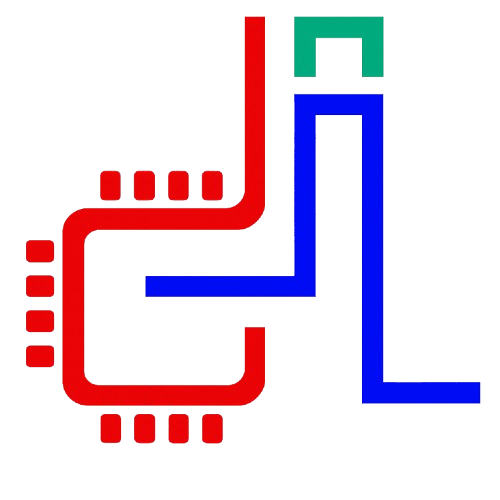
\includegraphics[width=1.25cm]{images/logo_department.png} \\
                    \textbf{Computer Science}\\
                    \textbf{Department}
                \end{center}
            \end{minipage}
        \end{center}
        
        \vspace{0.5cm}
        
        % Center section with title
        \begin{center}
            \textbf{\Large End of Studies Project Report}\\
            \vspace{1cm}
            \textbf{For the obtention of a National Engineering Diploma}\\
            \vspace{0.5cm}
            \textbf{Track: Software Engineering and Data Engineering}\\
            \vspace{1.5cm}
            \textit{Title:}\\
            \vspace{0.5cm}
            \textbf{\Huge PLAN GENIE AI}\\
            \vspace{0.2cm}
            \textbf{\Large Intelligent Task \& Event Management Platform}\\
            \vspace{0.2cm}
            \textbf{\large Powered by Advanced NLP and Speech Recognition}
        \end{center}
        
        \vspace{0.5cm}
        
        % Lower middle section with author and company
        \begin{center}
            \textit{Prepared by:}\\
            \vspace{0.5cm}
            \textbf{\Large Yassine Jedidi}\\
            \vspace{1cm}
            \textit{Realised within} \textbf{\large SFM}\\
            \vspace{0.5cm}
            
\includegraphics[width=5cm]{images/logo_entreprise.png}
        \end{center}
        
        \vspace{0.5cm}
        
        % Bottom section with supervisors and academic year
        \begin{center}
            \textit{Supervised by:}\\
            \vspace{0.5cm}
            \textbf{Ms. Amani Wattas (SFM)}\\
            \vspace{0.3cm}
            \textbf{Mr. Taoufik Ben Abdallah (FSB)}
        \end{center}
        
        \vfill
        
        % Bottom row with academic year
        \begin{center}
            \textbf{Academic Year 2024-2025}
        \end{center}
    \end{titlepage}
}

% Code listing setup
\lstset{
    basicstyle=\ttfamily\small,
    breaklines=true,
    frame=single,
    numbers=left,
    numberstyle=\tiny,
    keywordstyle=\color{blue},
    commentstyle=\color{green!60!black},
    stringstyle=\color{red},
    backgroundcolor=\color{gray!10},
    showstringspaces=false,
    tabsize=2
}

% Document begins
\begin{document}

% Cover page
\makecoverpage

% Dedication page
\newpage
\thispagestyle{empty}
\begin{center}
    \vspace*{5cm}
    \textbf{\Large Dedication}
    \vspace{2cm}
    
    \textit{To my family and mentors,}\\
    \textit{whose support made this possible.}
    \vfill
    
    \textit{--- Yassine Jedidi}
\end{center}

% Acknowledgements page
\newpage
\thispagestyle{empty}
\begin{center}
    \textbf{\Large Acknowledgements}
\end{center}

\vspace{1cm}

I would like to express my deepest gratitude to everyone who contributed to the successful completion of this project.

I extend my heartfelt thanks to my academic supervisor, Mr. Taoufik Ben Abdallah (FSB), for his expert guidance, constant support, and constructive feedback throughout every stage of this work.

I am especially grateful to my industrial supervisor, Ms. Amani Wattas (SFM), whose exceptional mentorship, technical expertise, and unwavering involvement were instrumental in shaping the direction and success of this project. Her commitment, availability, and deep understanding of the domain greatly enriched both the learning experience and the outcome of this work.

I also thank the SFM team for providing a supportive and inspiring environment, exposing me to real-world challenges, and entrusting me with responsibilities that made this AI-powered task and event management system possible.

I would like to express my appreciation to all my professors at the Faculty of Sciences of Bizerte for the education, support, and encouragement they have provided throughout my academic journey.

Finally, I express my sincere gratitude to my family for their unwavering support, patience, and understanding during this challenging journey. Their encouragement and belief in my abilities have been a constant source of motivation.

% Introduction page
\newpage
\thispagestyle{empty}
\begin{center}
    \textbf{\Large Introduction}
\end{center}

\vspace{1cm}

In today's busy world, managing tasks and events effectively is very important for both personal and work productivity. Traditional ways of managing tasks and events are often slow, make mistakes, and don't adapt to what users prefer.

This project introduces \textbf{Plan Genie AI}, a smart task and event management platform that uses artificial intelligence to change how people and organizations plan, organize, and track their activities. The system uses Natural Language Processing (NLP), speech recognition, and data analysis to provide a smooth, intelligent, and easy-to-use experience.

\vspace{0.5cm}

\textbf{Main Goals:}

\begin{itemize}
    \item Build an AI platform that can understand and process natural language for creating tasks and planning events
    \item Add speech-to-text features to allow voice-based task and event management
    \item Provide performance analytics and visualization tools
    \item Ensure data security and privacy protection
    \item Make a responsive application that works on different devices
\end{itemize}

\vspace{0.5cm}

The project uses modern technologies including React.js for the frontend, Node.js and Python FastAPI for backend services, PostgreSQL for data storage, and Hugging Face Transformers for advanced NLP features. The system can process multiple languages, extract information automatically, and provide detailed performance analytics through interactive charts.

\vspace{0.5cm}

This report shows the complete development process of Plan Genie AI, from initial idea and requirements through design, building, testing, and deployment. It demonstrates how artificial intelligence can be used to solve real productivity problems while maintaining good user experience and data security.

\newpage
\section{Preliminary Study}

\subsection*{Introduction}

The modern workplace and personal life demand efficient management of tasks and events. Traditional task management systems often fall short due to their rigid interfaces, limited automation capabilities, and lack of intelligent features. This chapter provides a comprehensive preliminary study of existing task and event management solutions, analyzing their strengths, limitations, and identifying market gaps that Plan Genie AI aims to address. Through this analysis, we establish the foundation for understanding current market limitations and opportunities for innovation in intelligent task and event management.

\section{Host Organization: SFM Technologies}
\subsection{General Overview}
Founded in 1995, \textbf{SFM Technologies} is a Tunisian consulting and engineering firm specializing in telecommunications, ICT, and digital transformation services. The company is part of the larger SFM Group, which includes subsidiaries such as SFM International, SFM Telecom, and SFM Cameroun. SFM operates in Africa, Europe, Asia, Oceania, and the United States.

\begin{figure}[H]
  \centering
  
\includegraphics[width=0.4\textwidth]{images/logo_entreprise.png}
  \caption{SFM Technologies Logo}
  \label{fig:sfm-logo}
\end{figure}

\subsection{Core Competencies}
SFM Technologies provides a wide array of services in the following areas:

\begin{itemize}
  \item \textbf{Telecommunications and Regulatory Support:} Benchmarking, audits, QoS/QoE analysis, and network planning for regulators and operators.
  \item \textbf{Strategic Engineering and Advisory:} Consulting on network convergence, privatization, spectrum regulation, and technology migration (e.g., analog to digital TV).
  \item \textbf{Training and Capacity Building:} Technical and theoretical training sessions in ICT and telecoms for institutions and companies.
  \item \textbf{R\&D and Software Development:} Through its R\&D branch, SFM Lab, the company creates custom software for fraud detection, tariff simulation, AI analytics, and network performance monitoring.
\end{itemize}

\subsection{Digital Tools and Platforms}
SFM Technologies develops and maintains several proprietary platforms:

\begin{itemize}
  \item Robotic Process Automation (e.g., COSAP, Ticketeazy, IT\&M)
  \item Cybersecurity Solutions (e.g., WiFi portal, PKI, SOC)
  \item AI and Big Data platforms for telecom, banking, and government sectors
  \item Modular software solutions tailored to specific client needs
\end{itemize}

\subsection{Clientele and Global Reach}
With a portfolio of over 30 clients, including national regulators, ministries, and international organizations such as the World Bank and African Development Bank, SFM Technologies has established itself as a trusted partner across several continents.

\subsection{Summary Table}

\begin{table}[H]
\centering
\begin{tabular}{|l|l|}
\hline
\textbf{Founded} & 1995 \\
\hline
\textbf{Legal Form} & SARL (R.C. 1028016M) \\
\hline
\textbf{Headquarters} & Tunis, Tunisia \\
\hline
\textbf{Core Areas} & Telecom regulation, digital transformation, ICT consulting and training \\
\hline
\textbf{R\&D Division} & SFM Lab \\
\hline
\textbf{Operational Presence} & Africa, Europe, Asia, Oceania, USA \\
\hline
\textbf{Main Offerings} & Consulting, audits, custom platforms, cybersecurity, AI solutions \\
\hline
\textbf{Clients} & Telecom operators, regulators, ministries, international donors \\
\hline
\end{tabular}
\caption{Summary of SFM Technologies' Key Information}
\end{table}

\section{Project Context and Problem Statement}

\subsection{Project Context}
The Plan Genie AI project emerged from a real-world need identified during the internship at SFM Technologies. The company, being a leading ICT consulting firm with operations across multiple continents, frequently deals with complex project management scenarios involving diverse teams, multilingual environments, and tight deadlines using their proprietary platform named COSAP. 

Recognizing the transformative potential of artificial intelligence, SFM Technologies sought to introduce AI-powered capabilities into their task and event management ecosystem. This strategic decision to leverage advanced AI technologies for enhanced productivity and intelligent automation ultimately led to the foundation of Plan Genie AI as a comprehensive, AI-driven task and event management platform.

\newpage
\textbf{Project Organization and Planning}

To ensure successful delivery of the Plan Genie AI platform, the project was structured into well-defined phases, each with specific objectives and deliverables. This systematic approach helps track progress, manage resources effectively, and ensure quality throughout the development process.

\textbf{Project Phases}
\begin{enumerate}
    \item \textbf{Phase 1: Conception} - Requirements analysis, system design, and architecture planning
    \item \textbf{Phase 2: Development} - Implementation of core features and AI integration
    \item \textbf{Phase 3: Tests and Validation} - Quality assurance and performance optimization
\end{enumerate}

\textbf{Project Deliverables}

The project produces several key deliverables that demonstrate the completion of objectives and provide value to both the development team and end users. These deliverables serve as milestones and evidence of project progress.

\textbf{Deliverables}
\begin{itemize}
    \item Functional and technical documentation
    \item Validated mockups and wireframes
    \item Complete and structured source code
    \item Functional application (web and mobile versions)
    \item Test reports and validations
\end{itemize}

\textbf{Project Constraints and Requirements}

Every project operates within certain boundaries and must meet specific requirements to be considered successful. Understanding these constraints and requirements is crucial for proper planning and execution.

\textbf{Constraints and Requirements}
\begin{itemize}
    \item \textbf{Multi-platform Compatibility:} Support for web, mobile, and desktop platforms
    \item \textbf{Performance and Scalability:} Efficient handling of large datasets and concurrent users
    \item \textbf{Data Security:} Implementation of robust security measures and data protection
    \item \textbf{Regulatory Compliance:} Adherence to relevant data protection and privacy regulations
    \item \textbf{Accessibility and Ergonomics:} User-friendly interface with accessibility features
\end{itemize}

\textbf{Project Timeline and Schedule}

Effective project management requires realistic time planning and scheduling. SFM Technologies defined a well planned and organized timeline. This timeline provided a roadmap for project execution and helps identify critical path activities that could impact overall project delivery.

\textbf{Estimated Timeline}
\begin{table}[H]
\centering
\begin{tabular}{|l|c|}
\hline
\textbf{Phase} & \textbf{Estimated Duration} \\
\hline
Conception & 4 weeks \\
\hline
Development & 16 weeks \\
\hline
Tests and Validation & 4 weeks \\
\hline
\textbf{Total} & \textbf{24 weeks (6 months)} \\
\hline
\end{tabular}
\caption{Project Timeline Overview}
\end{table}


\subsection{Problem Statement}

\textbf{Primary Problem}

The existing task and event management solutions available in the market fail to address the specific needs of modern, AI-driven organizations. Current tools lack the intelligence to automatically process natural language inputs, understand context, and provide meaningful insights for productivity optimization. This market gap and technological limitation explain why SFM Technologies wanted to develop Plan Genie AI - to create a comprehensive solution that addresses these critical shortcomings while leveraging advanced AI capabilities for enhanced productivity and intelligent automation.

The primary problem can be summarized as follows:

\textbf{How can artificial intelligence technologies be leveraged to create an intelligent task and event management platform that addresses the limitations of existing solutions while providing enhanced user experience, productivity optimization, and cross-platform accessibility?}



\textbf{Specific Challenges Identified}

\textbf{1. Market Gap in AI-Powered Task Management:}
The current market lacks comprehensive AI-driven task management solutions. Most existing tools rely on manual input and basic automation, failing to leverage advanced natural language processing and artificial intelligence capabilities that modern organizations require.

\textbf{2. Limited Natural Language Processing Capabilities:}
Existing solutions cannot intelligently process natural language inputs to automatically extract task details, deadlines, priorities, and contextual information. This limitation forces users to manually structure their thoughts into predefined formats, creating unnecessary friction.

\textbf{3. Insufficient Voice-Based Interaction Capabilities:}
Contemporary productivity tools should support voice input for accessibility and convenience. Existing solutions lack robust speech-to-text capabilities integrated with intelligent task management, limiting accessibility and user experience.

\textbf{4. Inadequate Analytics for Performance Optimization:}
Current tools provide only basic statistics and fail to offer actionable insights for improving productivity patterns, time management, and workflow optimization.

\section{Study and Critique of Existing Solutions}

To comprehensively understand the current landscape, we analyzed leading task and event management solutions across different categories and assessed them against criteria that matter for an AI-first, voice-enabled, multilingual platform.

\subsection{Scope and Method}
We grouped solutions into market segments, reviewed public documentation and hands-on usage, and evaluated capabilities along dimensions such as natural language handling, entity extraction, voice input, analytics and privacy. The goal is to identify where current tools excel, where they fall short, and what gaps remain for a next-generation solution.

\subsection{Market Segments}
\begin{itemize}
    \item \textbf{Traditional task managers}: Todoist, Microsoft To Do, Google Tasks, TickTick, Things 3, Any.do
    \item \textbf{Project/work management suites}: Asana, ClickUp, Jira, Trello, Monday.com
    \item \textbf{Calendar-centric tools}: Google Calendar, Outlook Calendar, Apple Calendar
    \item \textbf{AI-augmented assistants}: Notion (with Notion AI), ClickUp AI, Motion (AI scheduling)
\end{itemize}

\subsection{Evaluation Dimensions}
\begin{itemize}
    \item \textbf{Natural language understanding}: How well the tool parses free-form text for dates, priorities, and metadata
    \item \textbf{Entity extraction}: Ability to extract fields like date, time, location, context, and priority from a given input
    \item \textbf{Voice input quality}: Built-in speech capture, accuracy, latency, and how well it feeds into structured tasks/events
    \item \textbf{Data capture channels}: Variety and quality of inputs (text, file, voice) and how smoothly they convert into structured data
    \item \textbf{Natural Language Processing quality}: Accuracy of entity extraction (dates, deadlines, priorities, locations, participants) and task/event classification from text
    \item \textbf{Multilingual understanding of NLP}: Supported languages and equality of performance across them
    \item \textbf{Prioritization and scheduling intelligence}: Context-aware ordering scheduled tasks using deadlines and priorities
    \item \textbf{Notifications and reminders}: Customizable notifications that are scheduled in time and are useful to the user
    \item \textbf{UX and accessibility}: Responsive web and mobile experiences, multilingual UI, and accessibility compliance
    \item \textbf{Security and privacy}: Encryption, authentication posture, and adherence to regulations such as GDPR
    \item \textbf{Performance and latency}: Overall response time for speech recognition and NLP
    \item \textbf{Analytics and insights}: Depth of performance metrics and meaningful recommendations
    \item \textbf{Cross-platform usability}: Web, mobile, desktop, offline reliability, and accessibility
\end{itemize}

\subsection{Findings by Segment}
\textbf{Traditional task managers:}
\begin{itemize}
    \renewcommand\labelitemi{-}
    \item \textbf{Aligned}: Fast text capture (data capture), simple UX, good cross-platform support
    \item \textbf{Gaps}: Limited NLP/structuring quality, weak or no voice pipeline, basic analytics/reporting, minimal multilingual parity, shallow APIs
\end{itemize}

\textbf{Project/work management suites:}
\begin{itemize}
    \renewcommand\labelitemi{-}
    \item \textbf{Aligned}: Robust collaboration, workflows, integrations; decent analytics/reporting
    \item \textbf{Gaps}: Complexity; limited end-to-end NLP to structure; voice not native; prioritization/scheduling not context-aware enough; performance can degrade at scale
\end{itemize}

\textbf{Calendar-centric tools:}
\begin{itemize}
    \renewcommand\labelitemi{-}
    \item \textbf{Aligned}: Reliable scheduling, notifications, and ecosystem integration
    \item \textbf{Gaps}: Not task-first; weak NLP/structuring; limited analytics; no voice-to-structured pipeline; limited insights beyond events
\end{itemize}

\textbf{AI-augmented assistants:}
\begin{itemize}
    \renewcommand\labelitemi{-}
    \item \textbf{Aligned}: Text generation, summaries, some automation and insights
    \item \textbf{Gaps}: Inconsistent entity extraction for tasks/events; limited multilingual parity; voice capture not integrated into structured records; extensibility varies
\end{itemize}



\begin{table}[H]
\centering
\small
\begin{tabular}{|p{0.22\textwidth}|p{0.36\textwidth}|p{0.36\textwidth}|}
\hline
\textbf{Solution} & \textbf{Strengths} & \textbf{Limitations} \\
\hline
\textbf{Todoist} & Clean UI, cross-platform, natural language dates & Limited AI, no native voice pipeline to structured fields, basic analytics \\
\hline
\textbf{Notion} & Flexible workspace, powerful databases, collaborative & Not task-focused by default, setup complexity, AI not tailored to task structuring \\
\hline
\textbf{ClickUp} & Feature-rich, strong automation, customizable & Overwhelming for individuals, learning curve, AI add-ons are generic \\
\hline
\textbf{Microsoft To Do} & M365 integration, simple, shared lists & No advanced NLP, limited customization and analytics \\
\hline
\textbf{Asana} & Strong project management, timelines, integrations & Advanced features behind paid tiers, limited NLP/voice \\
\hline
\textbf{Jira} & Powerful workflows, Agile support, many plugins & Complex and heavy, steep learning curve, pricey for teams \\
\hline
\textbf{Trello} & Intuitive Kanban, many power-ups, simple tracking & Limited reporting/analytics, clutter at scale, minimal NLP \\
\hline
\textbf{Google Tasks} & Lightweight, Gmail/Calendar integration, fast & Very basic capabilities, no analytics, no AI/voice pipeline \\
\hline
\end{tabular}
\caption{Analysis of trending task and project management solutions (2025)}
\end{table}

\subsection{Key Gaps Observed}
\begin{itemize}
    \item \textbf{End-to-end NLP to structure}: Few tools reliably convert free text (or speech) into fully structured tasks/events with entities like date, time, location, participants, and priority
    \item \textbf{Voice-first capture}: Native, accurate speech-to-task pipelines are rare; voice is often detached from structured fields
    \item \textbf{Multilingual parity}: Many tools focus on English; robust multilingual understanding are limited
    \item \textbf{Task Prioritization:} Ineffective prioritization of tasks, leaving users uncertain about decisions and ultimately reducing productivity.
    \item \textbf{Performance and latency at scale}: Speech recognition and NLP can be slow or rate-limited in real-world loads
    \item \textbf{Actionable Analytics:} Dashboards are available, but there's little practical advice or feedback to help users improve their habits.
\end{itemize}

\subsection{Implications}
The market is mature in UI, collaboration, and basic automation, but it under-delivers on intelligent understanding, voice-native capture, multilingual capability, and adaptive insights. These gaps define where an AI-driven platform can meaningfully surpass market leaders by offering accurate NLP, robust speech pipelines, context-aware prioritization, and actionable analytics while maintaining strong privacy and extensibility.


\section{Proposed Solution and Objectives}

\subsection{Solution Overview}
Plan Genie AI addresses the identified market gaps by providing an intelligent, AI-powered task and event management platform that combines advanced Natural Language Processing, speech recognition, and data analytics to deliver a seamless user experience.

\subsection{Core Objectives}

\textbf{Primary Objectives:}
\begin{enumerate}
    \item Develop an intelligent task and event management system with \textit{Named Entity Recognition}
    \item Implement multilingual support for global accessibility optimally English and French
    \item Integrate speech-to-text functionality for voice-based interaction
    \item Provide intelligent task prioritization using AI algorithms
    \item Generate daily reports to view today's tasks and review past activities
    \item Deliver comprehensive analytics and performance tracking
    \item Ensure data security and privacy compliance
\end{enumerate}

\textbf{Secondary Objectives:}
\begin{enumerate}
    \item Create a responsive, cross-platform application
    \item Provide customizable notification and reminder systems
    \item Develop an intuitive user interface with modern design principles
    \item Implement internationalization to support multiple languages and locales
\end{enumerate}


\subsection{Key Differentiators}

\textbf{Advanced NLP Integration:}
Plan Genie AI leverages state-of-the-art Natural Language Processing models, including custom-trained Named Entity Recognition (NER) models, to automatically extract and categorize information from natural language inputs.

\textbf{Multilingual Capabilities:}
Unlike most existing solutions, Plan Genie AI supports multiple languages such as English and French, making it accessible to a global user base.

\textbf{Intelligent Prioritization:}
The system intelligently prioritizes tasks based on context, deadlines, and priorities.

\textbf{Comprehensive Analytics:}
Advanced data visualization and analytics provide users with insights into their productivity patterns, helping them optimize their workflow and time management.

\subsection{Comparative Analysis}

\begin{table}[H]
\centering
\resizebox{\textwidth}{!}{%
\begin{tabular}{|l|c|c|c|c|c|c|}
\hline
\textbf{Feature} & \textbf{Todoist} & \textbf{Google Calendar} & \textbf{Notion AI} & \textbf{ClickUp AI} & \textbf{Plan Genie AI} \\
\hline
Natural Language Processing & Basic & Limited & Advanced & Moderate & \textbf{Advanced} \\
\hline
Multilingual Support & Limited & Yes & Limited & Limited & \textbf{Yes} \\
\hline
Voice Input & No & No & No & No & \textbf{Yes} \\
\hline
AI-Powered Prioritization & No & No & No & Yes & \textbf{Yes} \\
\hline
Named Entity Recognition & No & No & No & Limited & \textbf{Yes} \\
\hline
Advanced Analytics & Basic & Basic & Moderate & Advanced & \textbf{Advanced} \\
\hline
Cross-Platform & Yes & Yes & Yes & Yes & \textbf{Yes} \\
\hline
Real-time Sync & Yes & Yes & Yes & Yes & \textbf{Yes} \\
\hline
Privacy Compliance & Basic & Advanced & Moderate & Advanced & \textbf{Advanced} \\
\hline
\end{tabular}%
}
\caption{Feature Comparison: Plan Genie AI vs. Existing Solutions}
\end{table}


\section{State of the Art on Named Entity Recognition Solutions}

\subsection{Introduction to Named Entity Recognition}

Named Entity Recognition (NER) is a critical task within Natural Language Processing (NLP) that involves the automatic identification and classification of textual entities into predefined categories such as person names, organizations, locations, dates, monetary values, and other domain-specific entities. NER serves as a foundational step for numerous downstream applications, including information retrieval, knowledge graph construction, question answering systems, and event extraction. In the realm of task and event management, NER significantly enhances system intelligence by enabling the extraction of actionable insights from unstructured natural language inputs, thereby improving automation and decision-making processes.

\begin{figure}[H]
  \centering
  \includegraphics[width=0.8\textwidth]{images/ner-introduction.png}
  \caption{Overview of Named Entity Recognition Process and Applications}
  \label{fig:ner-introduction}
\end{figure}

\subsection{Evolution of Traditional NER Approaches}

The development of NER methodologies has evolved through three distinct stages, each representing significant technological advancements in computational linguistics and pattern recognition.

\begin{figure}[H]
  \centering
  \includegraphics[width=0.9\textwidth]{images/ner-evolution.png}
  \caption{Evolution of Traditional NLP Approaches: From Rule-Based Systems to Neural Models}
  \label{fig:ner-evolution}
\end{figure}

\textbf{1. Rule-Based Systems}

Rule-based systems rely on manually crafted patterns and linguistic rules to identify entities. These systems use deterministic algorithms based on orthographic, syntactic, and lexical patterns.

\textbf{Example:} A rule might state: "If a word is capitalized and followed by 'Inc.' or 'Corp.', classify it as an ORGANIZATION." This approach works well in narrow domains but struggles with exceptions and new patterns.

\textbf{2. Statistical and Machine Learning Models}

The introduction of probabilistic models enabled systems to learn from annotated data rather than relying solely on manual rules.

\textbf{Conditional Random Fields (CRFs):} CRFs model label dependencies and contextual information jointly. For each word, they extract features like capitalization, orthographic patterns, and contextual words. CRFs consider the entire sequence, improving entity boundary detection.

\textbf{Support Vector Machines (SVMs):} SVM-based systems classify words individually based on extracted features, creating mathematical hyperplanes to separate entity types. They excel at binary classification tasks and handle high-dimensional feature spaces effectively.

\textbf{3. Neural Network-Based Models}

Deep learning introduced architectures capable of automatic feature extraction and representation learning.

\textbf{Bidirectional LSTM with CRF (BiLSTM-CRF):} This architecture combines bidirectional LSTM networks with CRF layers, representing the state-of-the-art in traditional NER approaches.

\textbf{Process:} Each word is converted to a vector representation, processed bidirectionally to capture context, and optimized through CRF layers for coherent tag sequences. This approach achieves 90-91\% F1 scores on standard benchmarks while maintaining computational efficiency and predictability.

\textbf{Key Advantages:}
\begin{itemize}
  \item \textbf{Precision:} High accuracy in known contexts with consistent 90-91\% F1 scores
  \item \textbf{Efficiency:} Lightweight compared to large language models, suitable for production environments
  \item \textbf{Predictability:} Deterministic behavior crucial for compliance-sensitive applications
  \item \textbf{Interpretability:} Maintains degree of interpretability through feature representations
\end{itemize}

This evolution demonstrates the continuous refinement from manual pattern matching to sophisticated neural architectures that automatically learn complex linguistic patterns while maintaining the reliability essential for production applications.

\subsection{LLM-Based NER Approaches}

The emergence of Large Language Models (LLMs) has revolutionized NER by introducing transformer-based architectures trained on massive text corpora. These models leverage pre-trained knowledge and contextual understanding to achieve superior performance in entity recognition tasks.

\textbf{1. Pretrained Transformers (BERT-style Models)}

Pretrained transformer models are trained on extensive unlabeled text through self-supervised objectives, enabling them to acquire deep linguistic knowledge before fine-tuning on specific NER tasks.

\textbf{Performance Advantages:} BERT-large models fine-tuned on standard benchmarks like CoNLL-2003 achieve approximately 92.8\% F1 scores, significantly outperforming traditional approaches. This improvement stems from contextual understanding—the model considers entire sentences rather than isolated words, enabling superior disambiguation of entity boundaries and meanings.

\textbf{Feature Learning:} A key advantage is the elimination of manual feature engineering. Transformers automatically learn rich, contextual representations that capture semantic relationships and linguistic patterns, reducing the need for domain-specific feature extraction.

\textbf{Key Transformer Variants:} Several transformer models have built upon BERT's architecture and training regimen:
\begin{itemize}
  \item \textbf{RoBERTa} \cite{liu2019roberta}: Reexamined BERT's training approach, employing dynamic masking, larger mini-batches, and more training data to boost model robustness and performance.
  \item \textbf{CamemBERT} \cite{martin2020camembert}: Adapted RoBERTa specifically for French, pretraining on a large-scale French corpus to enable superior performance on French NER benchmarks and multilingual applications.
  \item \textbf{XLM-RoBERTa} \cite{conneau2019unsupervised}: Extended RoBERTa to a multilingual setting by training on over 100 languages, enabling zero-shot and few-shot transfer for low-resource languages and cross-lingual NER tasks.
\end{itemize}

These pretrained models can be fine-tuned on annotated NER datasets with minimal task-specific architectural modifications, substantially reducing the need for extensive feature engineering. Moreover, the contextual embeddings generated by transformers provide rich semantic representations that help disambiguate entities in complex and ambiguous contexts.

\textbf{2. Generative LLMs (GPT-style Models)}

Modern generative models like GPT-3, GPT-4, and LLaMA introduce zero-shot and few-shot NER capabilities through instruction-following and text generation.

\textbf{Zero-Shot Capabilities:} These models can perform NER without task-specific training by following natural language instructions. For example, prompting "Extract all person names, locations, organizations, and dates from the following text" enables the model to identify entities based on its pre-trained knowledge.

\textbf{Flexibility:} Generative LLMs offer remarkable adaptability, allowing extraction of virtually any entity category through descriptive prompts, even for categories not present in traditional training schemas.

\textbf{Strengths of LLM-Based Approaches}

\textbf{Superior Accuracy:} Fine-tuned transformer models consistently achieve top-tier performance on standard benchmarks, excelling at complex linguistic phenomena including context understanding, entity disambiguation, and subtle cue recognition.

\textbf{Reduced Data Requirements:} Pre-training on billions of words enables effective performance with fewer labeled examples. Few-shot learning approaches can achieve competitive results with minimal or no additional training data.

\textbf{World Knowledge Integration:} LLMs incorporate extensive factual knowledge, enabling recognition of entities like "New York" as locations or "Acme Corp" as organizations without explicit training examples.

\textbf{Zero-Shot Flexibility:} The ability to perform NER without task-specific training makes these models suitable for rapid deployment and adaptation to new domains or entity types.

\textbf{Limitations and Challenges}

\textbf{Computational Cost:} LLMs require significant computational resources. BERT-base models with 110 million parameters are substantially heavier than traditional CRF models, while GPT-3 with 175 billion parameters demands extensive infrastructure.

\textbf{Inference Latency:} Processing speed can be a bottleneck, with models like GPT-3.5 taking seconds per input compared to traditional models processing thousands of tokens per second.

\textbf{Hallucination Tendencies:} LLMs may generate entities not explicitly present in the input text, such as expanding "JS" to "JavaScript," which can violate the principle of extracting exact text spans.

\textbf{Memory Requirements:} Deployment requires substantial RAM and GPU memory—several gigabytes for model weights compared to traditional models requiring only megabytes.

These LLM-based approaches represent the current state-of-the-art in NER, offering unprecedented accuracy and flexibility while introducing new considerations for computational efficiency and deployment constraints in production environments.



\subsection*{Conclusion}

This preliminary study established the context, motivations, and constraints that drive the development of Plan Genie AI. We analyzed the host organization and its ecosystem, articulated the problem statement and project objectives, and examined representative solutions across traditional, calendar-centric, and AI-powered tools. The comparative analysis highlighted clear gaps—particularly in multilingual NLP, integrated voice interaction, intelligent prioritization, and advanced analytics—that our platform is designed to address.

These findings validate the relevance of Plan Genie AI and provide a concrete foundation for the next steps. The upcoming chapter presents the detailed analysis, planning, and technological study that translate these insights into an actionable architecture, well-defined components, and an implementation roadmap aligned with the identified requirements and constraints.

\newpage
\section{Analysis, Planning, and Technological Study}

\subsection*{Introduction}
This chapter presents the requirements and architectural foundations of \textbf{Plan Genie AI}. We proceed step by step, starting with stakeholders and their interactions; subsequent sections (functional/non-functional requirements, use cases, planning, and detailed technological study) will follow in later subsections.

\section*{2.1 Requirements Gathering}
\subsection*{2.1.1 Identification of Actors}
\begin{itemize}
  \item \textbf{End User}: Authenticates, inputs text or voice, manages tasks/events, and consults analytics and dashboards.
  \item \textbf{Authentication Provider (Supabase)}: Manages user authentication (email/password and OAuth) and validates tokens.
  \item \textbf{NLP Service (FastAPI on Hugging Face)}: Classifies input (Task vs. Event) and extracts entities (title, deadline/date\_time, priority).
  \item \textbf{Voice Transcription Service (Groq Whisper)}: Transcribes uploaded audio files to text.
  \item \textbf{AI Prioritization Service (Google Gemini)}: Prioritizes active tasks and returns ordered lists with reasoning.
  \item \textbf{Database (PostgreSQL via Prisma)}: Persists users, tasks, events, bilans, and notifications.
  \item \textbf{Notification Subsystem}: Creates scheduled reminders for tasks and events at key horizons (1 day, 6h, 1h, 15m).
\end{itemize}

\subsection{Functional Requirements}
This subsection specifies the end-to-end capabilities that \textbf{Plan Genie AI} must offer to deliver value to users. Requirements are grouped by domain and reflect the implemented flows across the React frontend, Express backend, FastAPI NLP service, and third-party AI services.

\paragraph{Authentication and Account Management}\mbox{}

A secure, user-friendly authentication layer backed by Supabase~\cite{supabase}.
\begin{itemize}
  \item \textbf{Email/password auth}: Users sign up and sign in through validated web forms with clear, actionable feedback when inputs are invalid. Once authenticated, access to application pages is gated within the single-page app (SPA) to protect user data and actions. The flow is designed to remain intuitive while enforcing security best practices.
  \item \textbf{OAuth (Google)}: The application supports Google sign-in through a standards-based redirect and token exchange. After a successful exchange, the backend persists the session in secure cookies (\texttt{access-token} and \texttt{refresh-token}) so the user can navigate the app without re-entering credentials. This approach improves usability while preserving server-side control over sessions.
  \item \textbf{Cookies and Their Use}: Cookies are small pieces of data stored by the browser to maintain session state. HttpOnly cookies are inaccessible to JavaScript, protecting tokens from cross-site scripting (XSS) attacks. Cookies store access and refresh tokens securely, enable persistent login sessions, and manage authentication state across browser tabs and reloads.
  \item \textbf{Access and Refresh Tokens}: Access tokens are short-lived and used to authorize requests, minimizing risk if compromised. Refresh tokens have longer lifetimes and are securely stored in HttpOnly cookies, enabling seamless token renewal without user disruption. The backend validates refresh tokens to issue new access tokens, ensuring continuous secure sessions.
  \item \textbf{Session handling}: Sessions use HttpOnly cookies with appropriate SameSite settings to reduce exposure to client-side scripts and cross-site attacks. The backend validates tokens on every protected request so only legitimate sessions can access resources. This consistent check ensures that compromised or expired tokens cannot be used silently.
  \item \textbf{Sign-out and password flows}: Signing out explicitly clears authentication cookies so sessions end immediately across tabs. Password reset and change flows allow users to recover or rotate credentials whenever needed. These flows are integrated into the overall security posture to keep accounts protected.
  \item \textbf{Frontend guards}: The application uses a context/provider pattern to guard protected routes in the SPA. Pages on the platform only render when a valid session is present. This prevents accidental disclosure of private views and data.
  \item \textbf{Bot protection}: Cloudflare Turnstile challenges are applied on web sign-in and sign-up to reduce automated abuse. The flow remains unobtrusive for legitimate users (does not force the user to take extra or complicated steps) while adding a significant barrier against scripted attacks. This protection complements rate limiting and server-side checks.
  \item \textbf{Backend validation}: Middleware verifies tokens with the database before allowing access to any protected endpoint. This centralizes authorization logic and ensures consistent enforcement across controllers and services. It also simplifies maintenance by keeping checks in one place.
  \item \textbf{Cookie configuration}: Cookies use environment-aware domains and security flags such as SameSite=None and Secure in production. These settings ensure cross-site requests work where intended while keeping transport encrypted. Configuration remains flexible across local, staging, and production environments.
\end{itemize}

\paragraph{Multimodal Data Ingestion (Text and Voice)}\mbox{}

Seamless capture of user input as text or recorded audio.
\begin{itemize}
  \item \textbf{Text input (English/French)}: Users can enter free-form text in either English or French, and the system processes it consistently through the same downstream pipeline. This parity makes the experience predictable regardless of the user's preferred language. It also simplifies subsequent NLP processing and structuring.
  \item \textbf{File upload (text)}: Users can upload text files (for example, \texttt{.txt}) that the backend accepts as \texttt{multipart/form-data}. The server reads and normalizes the content to \texttt{UTF-8} and routes it through the same NLP pipeline as manual input so the resulting structure remains consistent. Size and type checks protect the service from oversized or unsupported files.
  \item \textbf{Audio capture}: Users record audio that the backend accepts as \texttt{multipart/form-data}. The backend proxies the audio to the transcription service and returns the recognized text to the client. This path provides an equivalent experience to text entry for voice-first users.
  \begin{center}
    \small\textit{-- \texttt{UTF-8} is a standard character encoding that can represent every character in Unicode, allowing consistent handling of text in multiple languages.}\\
    \small\textit{-- \texttt{multipart/form-data} is a special encoding type for forms that need to send files or binary data along with regular text fields (audio/wav in our case).}
    \end{center}
\end{itemize}


\paragraph{NLP Processing and Structuring}\mbox{}

Automatic classification and entity extraction to convert free-form input into structured records.
\begin{itemize}
  \item \textbf{Type classification}: The system detects whether an input describes a task or an event. This first step determines which fields are relevant and how the record should be created. It also helps the UI decide which form of feedback and next actions to present.
  \item \textbf{Entity extraction}: The NLP service extracts key fields such as Title, Deadline or Date/Time, and Priority. Extracted fields are then filtered according to the detected type so only relevant information is retained. This targeted filtering prevents noise from entering the database.
  \item \textbf{Tokenizer alignment}: Text inputs are tokenized using the same tokenizer as the underlying NER model to preserve token boundaries and improve accuracy. This alignment reduces mismatches between the raw text and model expectations. It contributes directly to better extraction quality.
  \item \textbf{Type-specific fields}: For a task, the structured output focuses on Title, Deadline, and Priority. For an event, the output focuses on Title and Date/Time. This clear mapping enables immediate creation or pre-filling of forms with minimal manual edits.
\end{itemize}


\paragraph{Task Management}\mbox{}

Comprehensive lifecycle management for tasks with prioritization context.
\begin{itemize}
  \item \textbf{Creation and editing}: Users can create tasks manually or from NER results, then adjust title, deadline, priority, and status as needed. This flexibility supports both quick capture and careful refinement. It also keeps tasks up to date as priorities change.
  \item \textbf{Lifecycle operations}: Users can list, update, and delete tasks during daily work. Completed tasks are excluded from prioritization so the system focuses on actionable items. The result is a cleaner, more relevant task list.
  \item \textbf{Time tracking linkage}: Each task can be linked to daily reporting entries to capture minutes spent and optional notes. This connection provides visibility into how time is allocated. It also powers analytics and performance insights.
  \item \textbf{UI sorting and filters}: The interface highlights high-priority tasks and items due soon so attention goes where it is needed most. Users can filter and sort to match their workflow. These affordances reduce cognitive load and improve execution.
\end{itemize}

\paragraph{Event Management}\mbox{}

Create and maintain calendar-oriented events.
\begin{itemize}
  \item \textbf{Creation and editing}: Users can create events manually or from NER analysis, then update titles and date/time fields. This supports both quick scheduling and careful adjustments. Events remain easy to review and modify over time.
  \item \textbf{Calendar integration}: The application lists, updates, and deletes events and renders them in calendar views. Visual placement on the calendar provides context and aids planning. The goal is to make event timelines obvious at a glance.
\end{itemize}

\paragraph{Intelligent Prioritization}\mbox{}

Leverage \texttt{Google Gemini} \cite{gemini2025flash} to order active tasks with transparent reasoning.
\begin{itemize}
  \item \textbf{Active-set focus}: The prioritization engine considers only active tasks and computes urgency indicators to determine order. This approach keeps results focused on what matters now. It also avoids clutter from completed items.
  \item \textbf{Explainable ordering}: The system returns a language-aware explanation in English or French that clarifies why tasks appear in a given sequence. These explanations improve trust and help users make better decisions. They also provide a learning loop for future refinements.
  \item \textbf{Urgency signals}: Days until deadline and similar cues inform the model's reasoning, including due-today or overdue annotations. Users can quickly understand which tasks require immediate action. The signals align the model's output with real-world urgency.
\end{itemize}

\paragraph{Notifications and Reminders}\mbox{}

Proactive alerts for upcoming deadlines and events.
\begin{itemize}
  \item \textbf{Advance reminders}: The system generates notifications at 1 day, 6 hours, 1 hour, and 15 minutes before due or start times for each task and event. These reminders help users prepare without constantly checking their schedule. They reduce the risk of missing critical moments.
  \item \textbf{Acknowledgement}: Users can mark notifications as read to acknowledge reminders and manage follow-up. Read states make it easy to separate new alerts from ones already handled. This creates a clear picture of what remains to be addressed.
  \item \textbf{Notification preferences}: Users can enable or disable notifications separately for tasks and events, customizing their alert experience to avoid overload or missed updates.

\end{itemize}

\paragraph{Daily Reporting}\mbox{}

Time tracking and daily summaries.
\begin{itemize}
  \item \textbf{Daily entries}: Users can consult daily reports showing tasks that can be worked today, as well as overdue tasks, and enrich tasks with entries that capture minutes spent and optional notes. This lightweight practice builds a reliable record of effort. It also helps users reflect on progress at the end of the day.
  \item \textbf{Review and edit}: Entries can be updated during or after the day to reflect actual effort. Corrections and additions keep the record accurate. Over time, these records power meaningful analytics.
  \item \textbf{History and access}: Users can consult recent daily reports to review their past work, track progress over time, and identify patterns in task completion.
\end{itemize}

\paragraph{Analytics and Dashboard}\mbox{}

Insight surfaces to improve productivity and planning.
\begin{itemize}
  \item \textbf{Charts and metrics}: The application visualizes completion rates, deadline adherence, and time distribution by task. These charts highlight patterns that are difficult to see in raw lists. They guide users toward better prioritization and planning.
  \item \textbf{KPIs and trends}: Key indicators summarize performance across a chosen time window (Today, This Week, This Month, All Period) so progress is easy to assess. Trend lines reveal whether productivity is improving or slipping. Users can then adjust behavior and goals accordingly.
\end{itemize}

\paragraph{Internationalization and Accessibility}\mbox{}

A globally usable and inclusive product experience.
\begin{itemize}
  \item \textbf{UI languages}: The interface supports runtime switching between English and French so users can work in their preferred language. System messages and labels follow the same setting to maintain consistency. This flexibility expands accessibility without fragmenting functionality.
  \item \textbf{NLP parity}: The NLP pipeline treats English and French inputs with the same care so structured fields remain consistent. Users can switch languages without losing capability or accuracy. The result is a smoother multilingual experience.
\end{itemize}

\paragraph{Error Handling and User Feedback}\mbox{}

Clear, actionable, and localized feedback for errors and long-running operations to maintain user trust.
\begin{itemize}
  \item \textbf{Frontend UX}: Forms validate inline, asynchronous actions use non-blocking spinners, and toasts communicate success or failure in English or French. Messages explain what happened and how to recover. This transparency reduces frustration and speeds resolution.
  \item \textbf{Network resiliency}: The app applies timeouts and retries for key API calls and degrades gracefully if NLP or transcription is temporarily unavailable. Users can continue with manual text input until services recover. This approach preserves momentum even during partial outages.
  \item \textbf{Actionable messages}: Error feedback surfaces precise causes such as authentication required, invalid input, rate limiting, or file size constraints. Each message suggests a concrete next step. Users spend less time guessing and more time moving forward.
  \item \textbf{Observability hooks}: The server logs request failures and unexpected conditions with enough context for diagnosis. Consistent error envelopes make client handling predictable. These practices support continuous improvement over time.
\end{itemize}

The functional requirements outlined above establish a comprehensive framework for \textbf{Plan Genie AI}'s core capabilities, ensuring that users can effectively manage tasks and events through intelligent, multimodal interactions while maintaining data integrity and system reliability.

\subsection{Non-Functional Requirements}
Building upon the functional capabilities outlined above, this subsection defines the quality attributes and operational constraints that ensure \textbf{Plan Genie AI} delivers a reliable, secure, and scalable user experience. These requirements guide design decisions across all system components and establish the foundation for production-ready deployment.

\begin{itemize}
  \item \textbf{Security}: Enforce secure authentication and data exchange using HttpOnly cookies with appropriate SameSite policies and HTTPS everywhere. Validate tokens on every protected endpoint via Supabase to prevent unauthorized access. Keep secrets only in environment variables and never expose them to the client, and restrict CORS to the intended frontend origin with explicit handling for preflight requests.

  \item \textbf{Privacy and Compliance}: Collect and process only the data that is necessary for functionality, and avoid storing raw audio beyond the transcription need. Obtain explicit consent for notifications, present a clear privacy policy, and document data usage transparently. Align behavior with \texttt{GDPR} principles including purpose limitation, data minimization, and user rights to access and erasure when applicable.
  \begin{center}
  \small\textit{\texttt{GDPR} (General Data Protection Regulation) is a European Union regulation that governs the collection, storage, and processing of personal data. It ensures individuals have rights over their data, including access, correction, and deletion, and obliges organizations to use data responsibly and transparently.}
  \end{center}


  \item \textbf{Performance and Latency}: Ensure the UI remains responsive by avoiding blocking operations and preloading necessary resources on application load to reduce startup delays. Optimize processing by caching results when safe and batching network calls to improve throughput, so users experience minimal delays.

  \item \textbf{Scalability}: Architect the backend to be stateless, enabling seamless horizontal scaling on serverless and cloud platforms. By avoiding server-side session dependencies, the system can efficiently distribute load across multiple instances, handle spikes in user traffic, and maintain high availability. Additionally, designing for scalability ensures that future growth and feature expansions can be accommodated without major architectural changes.


  \item \textbf{Reliability and Resilience}: Provide graceful fallbacks when external providers are unavailable so users can continue with manual flows. Apply timeouts and retries to critical calls and design for partial failure with clear error paths so that one degraded service does not halt the whole product experience.

  \item \textbf{Observability and Monitoring}: Log significant server events and errors with enough context to diagnose issues quickly. Keep a consistent error envelope across controllers and services so the client can handle failures predictably. Track the availability of external services to inform user-facing feedback and operational responses.

  \item \textbf{Maintainability and Code Quality}: Keep a layered architecture with clear separation of concerns across routes, controllers, services, middleware, and data access. Use TypeScript~\cite{typescript} on the frontend for safer refactoring and enforce linting and formatting for consistent style. Manage the schema in Prisma~\cite{prisma} as a single source of truth for models and relations.

  \item \textbf{Testability and QA}: Structure endpoints and services to be testable in isolation with deterministic logic and clear contracts on NLP proxy endpoints. Validate schemas at boundaries and return predictable error codes so automated tests can assert behavior and regressions are easy to catch.

  \item \textbf{Internationalization Quality}: Provide equal-quality handling for English and French at both the UI and NLP levels so structured outputs remain consistent. Maintain stable field mappings independent of language, and prevent language-specific regressions in entity extraction and prioritization explanations through focused testing.

  \item \textbf{Accessibility}: Support keyboard navigation, adequate color contrast, and screen-reader friendly components across authentication, tasks, events, and reporting. Make error messages perceivable and descriptive so users with assistive technologies can understand and complete key flows.

  \item \textbf{Data Integrity and Consistency}: Enforce referential integrity for tasks, events, daily reports, and notifications, and use UUIDs for stable identifiers. Normalize date and time storage and prefer \texttt{ISO-8601} at boundaries so data remains consistent across services and time zones.
  \begin{center}
  \small\textit{\texttt{ISO-8601} is an international standard for representing dates and times in a consistent format (e.g., YYYY-MM-DDTHH:MM:SSZ), which helps avoid ambiguity across different locales and time zones.}
  \end{center}

  \item \textbf{Configuration and Secrets Management}: Store secrets in environment variables outside of source control. Separate frontend-visible configuration from server-only values so sensitive data is never exposed.

  \item \textbf{Deployment and Environments}: Support local, staging, and production environments with environment-specific URLs and credentials, and keep deployments stable. Minimize cold-start impact on critical paths through warm-up strategies and careful resource initialization.

  \item \textbf{Interoperability and API Contracts}: Use REST and JSON with stable field names and status codes, and version endpoints cautiously. Document request and response shapes including error envelopes so integrations can be implemented and maintained with confidence over time.

  \item \textbf{Error Handling Policy}: Return meaningful HTTP codes and actionable messages without exposing internal stack traces. Wrap third-party errors in consistent, user-friendly responses so the client can display helpful guidance without leaking implementation details.

  \item \textbf{Backup and Recovery}: Enable managed database backups and define restoration procedures that preserve referential links between entities. Verify recovery plans periodically so data can be restored safely in the event of failure.

  \item \textbf{Time and Locale Handling}: Store timestamps in UTC and format them for display according to the user's locale. Indicate time zones clearly in the UI for events and deadlines so scheduling remains unambiguous across regions.

  \item \textbf{Browser and Device Support}: Target modern browsers on desktop and mobile, and degrade gracefully when APIs such as audio recording are unavailable. Offer alternative input flows so core tasks remain achievable across devices and environments.
\end{itemize}

These non-functional requirements establish the foundation for a production-ready system that prioritizes user experience, data security, and operational reliability. Together with the functional requirements, they provide a comprehensive framework for the system's design and implementation decisions.

\subsection{Global Use Case Diagram}

This section complements the scenario table with a consolidated view of how the \textit{User} interacts with \textbf{Plan Genie AI}. The diagram provides a single picture of the core capabilities and their dependencies across authentication, task and event management, prioritization, notifications, analytics, and settings.

Before examining the diagram, the following table summarizes the key user scenarios at a glance. It captures the intent behind each interaction and the outcome the user expects, serving as a compact reference for the flows depicted visually.

\begin{table}[H]
  \centering
  \small
  \begin{tabular}{|l|p{0.72\textwidth}|}
    \hline
    \textbf{Scenario} & \textbf{Description} \\
    \hline
    Sign In & User authenticates with email/password or Google OAuth to access protected features. \\
    \hline
    Sign Up & User creates an account with required fields; bot protection reduces automated abuse. \\
    \hline
    Reset Password & User requests a reset link and sets a new password to regain access securely. \\
    \hline
    Configure Settings & User updates theme, language, and notification preferences to personalize the experience. \\
    \hline
    Edit Profile & User edits personal information and avatar for identification within the app. \\
    \hline
    Create Task & User creates a task manually or from NLP output, setting title, deadline, and priority. \\
    \hline
    Create Event & User creates an event manually or from NLP output, setting title and date/time. \\
    \hline
    View Task \textbar{} Event & User browses lists and details, with options to sort and focus on relevant items. \\
    \hline
    Manage Task \textbar{} Event & User updates fields or deletes records that are no longer needed. \\
    \hline
    Filter Task \textbar{} Event & User filters by status, priority, or date to reduce cognitive load. \\
    \hline
    Prioritize Tasks & System orders active tasks using AI and presents reasoning to support decisions. \\
    \hline
    View Notification & User reviews upcoming reminders for tasks and events. \\
    \hline
    Mark Notification as Read & User acknowledges notifications to clear alerts and track follow-up. \\
    \hline
    View Analysis \textbar{} Dashboard & User explores KPIs, charts, and trends over selected periods. \\
    \hline
  \end{tabular}
  \caption{Key user scenarios in Plan Genie AI}
\end{table}

Before examining the diagram, the following table provides a comprehensive specification of all use cases in the system, detailing the actor interactions, objectives, flows, and expected outcomes for each functionality.

\begin{longtable}{|p{0.15\textwidth}|p{0.08\textwidth}|p{0.12\textwidth}|p{0.25\textwidth}|p{0.15\textwidth}|p{0.12\textwidth}|}
  \hline
  \textbf{Use Case} & \textbf{Actor} & \textbf{Objective} & \textbf{Main Flow} & \textbf{Alternative Flow} & \textbf{Postcondition} \\
  \hline
  \endfirsthead
  
  \multicolumn{6}{c}%
  {\tablename\ \thetable\ -- \textit{Continued from previous page}} \\
  \hline
  \textbf{Use Case} & \textbf{Actor} & \textbf{Objective} & \textbf{Main Flow} & \textbf{Alternative Flow} & \textbf{Postcondition} \\
  \hline
  \endhead
  
  \hline \multicolumn{6}{|r|}{\textit{Continued on next page}} \\
  \endfoot
  
  \hline
  \endlastfoot
  
  Sign In & User & Authenticate user and grant system access & User provides credentials. System validates and authenticates user. & Invalid credentials; Account locked; Password expired & User is authenticated and logged in \\
  \hline
  Sign Up & User & Create new user account & User provides registration details. System validates and creates account. & Invalid information; Email already exists & New user account is created \\
  \hline
  Reset Password & User & Reset account password & User requests reset. System sends verification. User sets new password. & Invalid reset token; Expired link & User's password is reset \\
  \hline
  Configure Settings & User & Customize application settings & User accesses settings. System displays current settings. User modifies preferences. & Invalid settings format & User's settings are updated \\
  \hline
  Edit Profile & User & Modify personal profile information & User accesses profile. System displays current details. User updates fields. & Invalid profile data & User's profile is updated \\
  \hline
  View Notification & User & View system notifications & User accesses notification area. System retrieves and displays notifications. & No notifications available & Notifications are displayed \\
  \hline
  Mark Notification as Read & User & Mark notification as read & User selects notification. System updates status to 'read'. & Notification already read & Notification status is updated \\
  \hline
  Prioritize Tasks & User & Set or change task priorities & User accesses task list. User selects tasks and assigns priority. & No tasks available & Task priorities are updated \\
  \hline
  Create Task & User & Create new task entry & User initiates creation. User provides task details. System validates and saves. & Invalid task data & New task is created \\
  \hline
  Create Event & User & Create new event entry & User initiates creation. User provides event details. System validates and saves. & Invalid event data & New event is created \\
  \hline
  View Task \textbar{} Event & User & View existing tasks or events & User requests view. System retrieves and displays list. & No tasks/events available & Tasks/events are displayed \\
  \hline
  Manage Task \textbar{} Event & User & Edit or delete tasks/events & User selects item. User chooses action. System performs operation. & Item not found & Task/event is modified/deleted \\
  \hline
  Filter Task \textbar{} Event & User & Filter displayed items by criteria & User applies filter criteria. System re-displays filtered results. & No matching items & Filtered results are displayed \\
  \hline
  View Analysis \textbar{} Dashboard & User & View analytical data and dashboard & User accesses analysis section. System retrieves and displays data. & No data available & Analytics and dashboard are displayed \\
  \hline
  \caption{Use Case Specification Table for Plan Genie AI}
\end{longtable}

\begin{figure}[H]
  \centering
  \includegraphics[width=0.95\textwidth]{images/Use Case.jpg}
  \caption{Global Use Case Diagram for Plan Genie AI}
  \label{fig:usecase}
\end{figure}

In short, the diagram ties the scenarios together: authentication unlocks protected actions, task and event creation flows into viewing and optional management or filtering, prioritization orders active tasks with explanations, notifications can be reviewed and acknowledged, and analytics provides feedback loops for planning. This shared view aligns navigation, authorization, and data relationships for the next sections.

\section{Project Planning}

To structure our approach, we adopted two complementary frameworks: \textbf{CRISP–DM} to guide the logic of the AI project and \textbf{Kanban} to organize work in an \texttt{Agile}, flow‑based manner. This combination provides both a rigorous structure for the deep learning lifecycle and a visual, flexible management of day‑to‑day activities. While CRISP–DM frames the major stages—from business understanding through deployment—Kanban enables continuous tracking, fast adaptation when surprises occur, and dynamic prioritization. The hybrid approach improves collaboration, reduces blockers, and supports continuous improvement across the development cycle of AI‑powered solutions.

\small\textit{\texttt{Agile} is a methodology focused on iterative development, flexibility, and collaboration. It emphasizes delivering small, incremental improvements frequently, responding to change quickly, and involving team members throughout the process to ensure solutions meet real needs.}


\subsection{CRISP–DM Model}

The CRISP-DM framework consists of six interconnected phases that form an iterative development cycle 
\begin{itemize}
  \item \textbf{Business Understanding}: Focuses on understanding project objectives and requirements from a business perspective, then converting this knowledge into a data mining problem definition and preliminary project plan.
  \item \textbf{Data Understanding}: Involves initial data collection and exploration to familiarize with the data, identify data quality problems, discover first insights into the data, and detect interesting subsets.
  \item \textbf{Data Preparation}: Covers all activities required to construct the final dataset from initial raw data, including data selection, cleaning, construction, integration, and formatting.
  \item \textbf{Modeling}: Involves selecting and applying various modeling techniques, calibrating their parameters to optimal values, and considering multiple approaches when appropriate.
  \item \textbf{Evaluation}: Thoroughly evaluates the model and reviews the steps executed to construct it, ensuring the model properly achieves business objectives before deployment.
  \item \textbf{Deployment}: Involves organizing and presenting findings in a way that stakeholders can use, from generating reports to implementing repeatable data mining processes.
\end{itemize}

\begin{figure}[H]
  \centering
  \includegraphics[width=0.9\textwidth]{img/CRISP-DM.png}
  \caption{CRISP–DM framework and iterative lifecycle}
  \label{fig:crispdm}
\end{figure}

\subsection{Kanban Method}

Kanban encourages breaking work into small, independently valuable tasks. Instead of time‑boxed sprints, the team continuously pulls the highest‑priority item from the backlog when capacity is available. A Kanban board visualizes flow with columns such as \textit{To Do}, \textit{In Progress}, \textit{Review/QA}, and \textit{Done}. Cards move across columns, making status and bottlenecks immediately visible. Work‑In‑Progress limits reduce multitasking, while explicit policies (Definition of Ready/Done) keep quality predictable. Benefits include stronger customer satisfaction via shorter cycle times, clear process visualization, empowered self‑management, rapid identification of blockers, flexible prioritization, and effective coordination of interdependent tasks. For this project, a Kanban board was maintained in \textit{Trello} for daily tracking and prioritization.

\begin{figure}[H]
  \centering
  \includegraphics[width=0.95\textwidth]{img/Kanban.png}
  \caption{Kanban Methodology}
  \label{fig:kanban}
\end{figure}

\subsection{Functional Decomposition and Task Steering}

The following table synthesizes the main functionalities and the corresponding tasks to be carried out within our project. It bridges high‑level requirements and concrete backlog items used on the Kanban board.


\begin{longtable}{|l|p{0.72\textwidth}|}
  \hline
  \textbf{Functionality} & \textbf{Representative Tasks} \\
  \hline
  \endfirsthead
  
  \multicolumn{2}{c}%
  {\tablename\ \thetable\ -- \textit{Continued from previous page}} \\
  \hline
  \textbf{Functionality} & \textbf{Representative Tasks} \\
  \hline
  \endhead
  
  \hline \multicolumn{2}{|r|}{\textit{Continued on next page}} \\
  \endfoot
  
  \hline
  \endlastfoot
  
  Authentication & \begin{tabular}[t]{@{}l@{}}- Configure Supabase auth with email/password and Google OAuth \\ - Implement secure HttpOnly cookie strategy with access/refresh tokens \\ - Build protected route middleware \\ - Create sign-in/up/reset UI flows \\ - Integrate Turnstile bot protection \\ - Implement token refresh and rotation logic\end{tabular} \\
  \hline
  User Profile & \begin{tabular}[t]{@{}l@{}}- Design profile edit interface \\ - Implement avatar upload and storage \\ - Create theme and color theme persistence \\ - Build notification preference toggles \\ - Add user settings page with language and privacy controls\end{tabular} \\
  \hline
  Multimodal Ingestion & \begin{tabular}[t]{@{}l@{}}- Build text input with real-time validation \\ - Implement text file upload (\texttt{.txt}) with UTF-8 normalization \\ - Create audio recording interface with format validation \\ - Design audio upload via \texttt{multipart/form-data} \\ - Implement wake-up calls to Hugging Face Space \\ - Add file size and type restrictions\end{tabular} \\
  \hline
  NLP Pipeline & \begin{tabular}[t]{@{}l@{}}- Create proxy endpoints (\texttt{/api/predict-type}, \texttt{/api/extract-entities}, \texttt{/api/analyze-text}) \\ - Implement language detection for EN/FR \\ - Build type-specific entity filtering logic \\ - Add fallback date parsing \\ - Design consistent output schema \\ - Implement error handling for NLP service failures\end{tabular} \\
  \hline
  Task Management & \begin{tabular}[t]{@{}l@{}}- Design Prisma schema for tasks with relations \\ - Implement CRUD operations with optimistic UI updates \\ - Build status transition logic \\ - Create priority normalization \\ - Add timezone-aware deadline handling \\ - Implement filters for due-soon/high-priority views \\ - Link tasks to daily reports\end{tabular} \\
  \hline
  Event Management & \begin{tabular}[t]{@{}l@{}}- Design Prisma schema for events \\ - Implement CRUD with calendar integration \\ - Build date/time parsing with locale awareness \\ - Create calendar visualization components \\ - Add notification scheduling for event start times \\ - Implement edit/delete workflows\end{tabular} \\
  \hline
  AI Prioritization & \begin{tabular}[t]{@{}l@{}}- Integrate Google Gemini API with proper error handling \\ - Implement urgency computation algorithms \\ - Build rationale generation in EN/FR \\ - Create UI for displaying ordered tasks with explanations \\ - Add user override capabilities \\ - Implement commit/cancel behavior \\ - Add lightweight result caching\end{tabular} \\
  \hline
  Notification System & \begin{tabular}[t]{@{}l@{}}- Design notification schema with task/event relations \\ - Implement scheduling for 1d/6h/1h/15m reminders \\ - Build read state persistence \\ - Create user preference toggles \\ - Implement background refresh hooks \\ - Add notification center UI with filtering\end{tabular} \\
  \hline
  Daily Reports & \begin{tabular}[t]{@{}l@{}}- Design bilan schema with task relations \\ - Create today/overdue view \\ - Implement daily entry creation with minutes and notes \\ - Build recent history interface \\ - Add daily roll-up summaries \\ - Implement optional CSV export functionality\end{tabular} \\
  \hline
  Analytics Dashboard & \begin{tabular}[t]{@{}l@{}}- Design KPI queries for completion rates and deadline adherence \\ - Implement time distribution charts \\ - Create period selectors (Today/Week/Month/All) \\ - Build workload trend visualization \\ - Add performance metrics aggregation \\ - Implement interactive chart components\end{tabular} \\
  \hline
  Internationalization & \begin{tabular}[t]{@{}l@{}}- Configure i18next with EN/FR translations \\ - Implement runtime language switching \\ - Verify UI string consistency across languages \\ - Ensure AI outputs maintain language parity \\ - Add date/number localization \\ - Implement RTL support considerations\end{tabular} \\
  \hline
  Data Model & \begin{tabular}[t]{@{}l@{}}- Design comprehensive Prisma schema with User/Task/Event/Bilan/Notification models \\ - Implement UUID primary keys and foreign key relations \\ - Create database migrations \\ - Establish referential integrity and cascading rules \\ - Implement data validation constraints\end{tabular} \\
  \hline
  Security & \begin{tabular}[t]{@{}l@{}}- Implement CORS policy configuration \\ - Set secure cookie flags (Secure/SameSite/HttpOnly) \\ - Add server-side token validation middleware \\ - Implement minimal audio data retention \\ - Create privacy policy pages \\ - Add consent management interfaces\end{tabular} \\
  \hline
  Observability & \begin{tabular}[t]{@{}l@{}}- Design structured error envelope format \\ - Implement comprehensive server logging with context \\ - Create health check endpoints for API, DB, and NLP services \\ - Build user-friendly error message system \\ - Add performance monitoring hooks\end{tabular} \\
  \hline
  Deployment & \begin{tabular}[t]{@{}l@{}}- Configure Vercel projects for frontend and backend \\ - Deploy FastAPI service on Hugging Face Space \\ - Implement environment variable management \\ - Create post-deploy smoke tests and health checks \\ - Establish rollback procedures \\ - Set up monitoring and alerting\end{tabular} \\
  \hline
  \caption{Mapping of functionalities to representative implementation tasks}
\end{longtable}


This planning approach ensured that ML quality gates from CRISP–DM were honored without slowing delivery, while Kanban kept the team focused on the highest‑value, ready‑to‑ship work at all times.

This comprehensive planning approach successfully bridged the gap between high-level requirements and concrete implementation tasks. The hybrid CRISP-DM and Kanban methodology provided the structured framework needed for AI model development while maintaining the flexibility required for rapid iteration and adaptation. The detailed task decomposition ensured that each functionality was broken down into manageable, testable components that could be tracked and prioritized effectively throughout the development cycle. This systematic approach was instrumental in delivering a complex AI-powered task and event management platform that meets both functional requirements and quality standards within the project timeline.

% Next: 2.4 Technological Study (to be added)
% 2.4.1 Tools and Software Environments
% 2.4.2 System Architecture
% - Global Architecture
% - Physical Architecture
% - Logical Architecture

\section{Technological Study}

This section provides a comprehensive overview of the technological foundations that power \textbf{Plan Genie AI}. We examine the complete technology stack, development environments, deployment strategies, and third-party integrations that enable the platform's intelligent capabilities and robust performance.

\subsection{Tools and Software Environments}

The development of \textbf{Plan Genie AI} required a carefully selected technology stack that balances modern development practices with production-ready reliability. Our choice of technologies reflects the need for rapid iteration, scalable architecture, and seamless integration of AI services.

\subsubsection{Technology Stack Overview}

The platform is built using a modern, multi-platform architecture that supports web, mobile, and AI services. This comprehensive approach enables cross-platform development, independent scaling, and seamless integration of intelligent features across all user touchpoints.

\textbf{Web Frontend Layer:}
\begin{itemize}
  \item \textbf{React.js} - Modern JavaScript library for building user interfaces with component-based architecture and virtual DOM for optimal performance
  \begin{figure}[H]
    \centering
    \includegraphics[width=0.15\textwidth]{images/react-logo.png}
    \caption{React.js Logo}
  \end{figure}
  
  \item \textbf{TypeScript} - Superset of JavaScript providing static type checking, enhanced IDE support, and improved code maintainability
  \begin{figure}[H]
    \centering
    \includegraphics[width=0.15\textwidth]{images/typescript-logo.png}
    \caption{TypeScript Logo}
  \end{figure}
  
  \item \textbf{Vite} - Next-generation build tool offering lightning-fast hot module replacement and optimized production builds
  \begin{figure}[H]
    \centering
    \includegraphics[width=0.15\textwidth]{images/vite-logo.png}
    \caption{Vite Logo}
  \end{figure}
  
  \item \textbf{Tailwind CSS} - Utility-first CSS framework enabling rapid UI development with pre-built responsive components
  \begin{figure}[H]
    \centering
    \includegraphics[width=0.15\textwidth]{images/tailwind-logo.png}
    \caption{Tailwind CSS Logo}
  \end{figure}
  
  \item \textbf{Shadcn UI} - Modern component library built on Radix UI primitives providing accessible, customizable components with consistent design system
  \begin{figure}[H]
    \centering
    \includegraphics[width=0.15\textwidth]{images/shadcn-logo.png}
    \caption{Shadcn UI Logo}
  \end{figure}
\end{itemize}

\textbf{Mobile Development Layer:}
\begin{itemize}
  \item \textbf{React Native} - Cross-platform mobile application framework enabling development of native mobile apps for iOS and Android using JavaScript and React
  \begin{figure}[H]
    \centering
    \includegraphics[width=0.15\textwidth]{images/react-native-logo.png}
    \caption{React Native Logo}
  \end{figure}
  
  \item \textbf{Expo} - Development platform and framework for React Native providing tools, services, and SDKs for rapid mobile app development and deployment
  \begin{figure}[H]
    \centering
    \includegraphics[width=0.15\textwidth]{images/expo-logo.png}
    \caption{Expo Logo}
  \end{figure}
  
  \item \textbf{NativeWind} - Tailwind CSS implementation for React Native enabling utility-first styling and responsive design in mobile applications
  \begin{figure}[H]
    \centering
    \includegraphics[width=0.15\textwidth]{images/nativewind-logo.png}
    \caption{NativeWind Logo}
  \end{figure}
  
  \item \textbf{Expo Router} - File-based routing system for React Native applications providing declarative navigation and deep linking capabilities
  \begin{figure}[H]
    \centering
    \includegraphics[width=0.15\textwidth]{images/expo-router-logo.png}
    \caption{Expo Router Logo}
  \end{figure}
  
  \item \textbf{React Native Reanimated} - Advanced animation library for React Native providing smooth, native-driven animations and gesture-based interactions for enhanced mobile user experience
  \begin{figure}[H]
    \centering
    \includegraphics[width=0.15\textwidth]{images/react-native-reanimated-logo.png}
    \caption{React Native Reanimated Logo}
  \end{figure}
\end{itemize}

\textbf{Backend Services Layer:}
\begin{itemize}
  \item \textbf{Node.js} - JavaScript runtime environment enabling server-side development with non-blocking I/O and event-driven architecture
  \begin{figure}[H]
    \centering
    \includegraphics[width=0.15\textwidth]{images/nodejs-logo.png}
    \caption{Node.js Logo}
  \end{figure}
  
  \item \textbf{Express.js} - Minimal and flexible web application framework providing robust routing, middleware support, and RESTful API capabilities
  \begin{figure}[H]
    \centering
    \includegraphics[width=0.15\textwidth]{images/express-logo.png}
    \caption{Express.js Logo}
  \end{figure}
  
  \item \textbf{Python FastAPI} - High-performance web framework for building APIs with automatic documentation and async support
  \begin{figure}[H]
    \centering
    \includegraphics[width=0.15\textwidth]{images/fastapi-logo.png}
    \caption{FastAPI Logo}
  \end{figure}
  
  \item \textbf{Uvicorn} - Lightning-fast ASGI server implementation for running FastAPI applications with high performance and concurrency
  \begin{figure}[H]
    \centering
    \includegraphics[width=0.15\textwidth]{images/uvicorn-logo.png}
    \caption{Uvicorn Logo}
  \end{figure}
\end{itemize}

\textbf{AI/ML Intelligence Layer:}
\begin{itemize}
  \item \textbf{Hugging Face Transformers} - State-of-the-art natural language processing library with pre-trained models for text classification and entity recognition
  \begin{figure}[H]
    \centering
    \includegraphics[width=0.15\textwidth]{images/huggingface-logo.png}
    \caption{Hugging Face Logo}
  \end{figure}
  
  \item \textbf{CamemBERT} - French language model optimized for French NLP tasks including named entity recognition and text classification
  \begin{figure}[H]
    \centering
    \includegraphics[width=0.15\textwidth]{images/camembert-logo.png}
    \caption{CamemBERT Logo}
  \end{figure}
  
  \item \textbf{Google Gemini AI} - Advanced language model for intelligent task prioritization and natural language reasoning
  \begin{figure}[H]
    \centering
    \includegraphics[width=0.15\textwidth]{images/gemini-logo.png}
    \caption{Google Gemini AI Logo}
  \end{figure}
  
  \item \textbf{PyTorch} - Open-source machine learning framework providing tensor computations and deep learning capabilities for NLP models
  \begin{figure}[H]
    \centering
    \includegraphics[width=0.15\textwidth]{images/pytorch-logo.png}
    \caption{PyTorch Logo}
  \end{figure}
\end{itemize}

\textbf{Data Management Layer:}
\begin{itemize}
  \item \textbf{PostgreSQL} - Advanced open-source relational database system offering ACID compliance, extensibility, and robust performance
  \begin{figure}[H]
    \centering
    \includegraphics[width=0.15\textwidth]{images/postgresql-logo.png}
    \caption{PostgreSQL Logo}
  \end{figure}
  
  \item \textbf{Prisma ORM} - Next-generation database toolkit offering type-safe database access, automatic migrations, and powerful query capabilities
  \begin{figure}[H]
    \centering
    \includegraphics[width=0.15\textwidth]{images/prisma-logo.png}
    \caption{Prisma ORM Logo}
  \end{figure}
  
  \item \textbf{Supabase} - Open-source Firebase alternative providing PostgreSQL database, authentication, and real-time subscriptions
  \begin{figure}[H]
    \centering
    \includegraphics[width=0.15\textwidth]{images/supabase-logo.png}
    \caption{Supabase Logo}
  \end{figure}
\end{itemize}

\textbf{Deployment & Infrastructure Layer:}
\begin{itemize}
  \item \textbf{Vercel} - Cloud platform for static sites and serverless functions with global edge network and automatic deployments
  \begin{figure}[H]
    \centering
    \includegraphics[width=0.15\textwidth]{images/vercel-logo.png}
    \caption{Vercel Logo}
  \end{figure}
  
  \item \textbf{Hugging Face Space} - Platform for hosting machine learning models and applications with GPU acceleration and easy deployment
  \begin{figure}[H]
    \centering
    \includegraphics[width=0.15\textwidth]{images/huggingface-space-logo.png}
    \caption{Hugging Face Space Logo}
  \end{figure}
  
  \item \textbf{Expo Application Services} - Cloud services for React Native apps including builds, updates, and analytics
  \begin{figure}[H]
    \centering
    \includegraphics[width=0.15\textwidth]{images/expo-eas-logo.png}
    \caption{Expo EAS Logo}
  \end{figure}
\end{itemize}

\textbf{Development Tools Layer:}
\begin{itemize}
  \item \textbf{Visual Studio Code} - Integrated development environment providing advanced code editing, debugging, and extension ecosystem
  \begin{figure}[H]
    \centering
    \includegraphics[width=0.15\textwidth]{images/vscode-logo.png}
    \caption{Visual Studio Code Logo}
  \end{figure}
  
  \item \textbf{Git} - Distributed version control system enabling efficient tracking of code changes, branching, and collaborative development workflows
  \begin{figure}[H]
    \centering
    \includegraphics[width=0.15\textwidth]{images/git-logo.png}
    \caption{Git Logo}
  \end{figure}
  
  \item \textbf{GitHub} - Cloud-based hosting platform for Git repositories providing collaboration features, issue tracking, and continuous integration capabilities
  \begin{figure}[H]
    \centering
    \includegraphics[width=0.15\textwidth]{images/github-logo.png}
    \caption{GitHub Logo}
  \end{figure}
  
  \item \textbf{ESLint \& Prettier} - Code quality tools for linting and formatting ensuring consistent code style across web and mobile codebases
  \begin{figure}[H]
    \centering
    \includegraphics[width=0.15\textwidth]{images/eslint-prettier-logo.png}
    \caption{ESLint \& Prettier Logo}
  \end{figure}
  
  \item \textbf{Google Colab} - Cloud-based Jupyter notebook environment providing free GPU and TPU access for machine learning development and collaborative AI model training
  \begin{figure}[H]
    \centering
    \includegraphics[width=0.15\textwidth]{images/google-colab-logo.png}
    \caption{Google Colab Logo}
  \end{figure}
  
  \item \textbf{StarUML} - Professional UML modeling tool providing comprehensive diagram creation capabilities for software architecture design, class diagrams, sequence diagrams, and system modeling
  \begin{figure}[H]
    \centering
    \includegraphics[width=0.15\textwidth]{images/staruml-logo.png}
    \caption{StarUML Logo}
  \end{figure}
  
  \item \textbf{Docker} - Containerization platform enabling consistent application deployment across different environments with isolated dependencies and reproducible builds
  \begin{figure}[H]
    \centering
    \includegraphics[width=0.15\textwidth]{images/docker-logo.png}
    \caption{Docker Logo}
  \end{figure}
\end{itemize}

\textbf{UI/UX & Utilities Layer:}
\begin{itemize}
  \item \textbf{Radix UI} - Low-level UI primitives providing accessible, unstyled components that serve as the foundation for Shadcn UI
  \begin{figure}[H]
    \centering
    \includegraphics[width=0.15\textwidth]{images/radix-ui-logo.png}
    \caption{Radix UI Logo}
  \end{figure}
  
  \item \textbf{Axios} - Promise-based HTTP client for making API requests with automatic JSON transformation and interceptors
  \begin{figure}[H]
    \centering
    \includegraphics[width=0.15\textwidth]{images/axios-logo.png}
    \caption{Axios Logo}
  \end{figure}
  
  \item \textbf{i18next} - Internationalization framework enabling multi-language support across web and mobile platforms
  \begin{figure}[H]
    \centering
    \includegraphics[width=0.15\textwidth]{images/i18next-logo.png}
    \caption{i18next Logo}
  \end{figure}
  
  \item \textbf{Zod} - TypeScript-first schema validation library providing runtime type checking and automatic type inference
  \begin{figure}[H]
    \centering
    \includegraphics[width=0.15\textwidth]{images/zod-logo.png}
    \caption{Zod Logo}
  \end{figure}
\end{itemize}

\begin{figure}[H]
  \centering
  \includegraphics[width=0.9\textwidth]{images/tech-stack.png}
  \caption{Technology Stack Architecture Overview}
  \label{fig:tech-stack}
\end{figure}

\subsubsection{Development Environment Setup}

The development environment is designed to provide a consistent, reproducible setup that enables rapid iteration and collaborative development. Each component of the stack has been configured to work seamlessly together while maintaining clear separation of concerns.

\textbf{Frontend Development Environment:}
\begin{itemize}
  \item \textbf{React Development Server}: Vite provides hot module replacement and fast refresh capabilities, enabling instant feedback during development. The development server runs on \texttt{localhost:5173} with automatic port detection and fallback.
  \item \textbf{TypeScript Configuration}: Strict type checking is enabled to catch potential errors early. The configuration includes path mapping for clean imports and module resolution for third-party libraries.
  \item \textbf{Tailwind CSS}: Utility-first CSS framework with custom configuration for design tokens, responsive breakpoints, and component variants. The build process optimizes CSS for production by purging unused styles.
  \item \textbf{Component Library}: Shadcn UI provides a consistent design system with accessible, customizable components. The library is configured with a custom theme that matches the application's visual identity.
\end{itemize}

\textbf{Backend Development Environment:}
\begin{itemize}
  \item \textbf{Node.js Runtime}: Version 18.x provides modern JavaScript features including top-level await, enhanced performance, and improved debugging capabilities. The runtime is configured with appropriate memory limits and garbage collection settings.
  \item \textbf{Express.js Framework}: Configured with middleware for CORS, body parsing, cookie handling, and file uploads. The application structure follows MVC patterns with clear separation between routes, controllers, and services.
  \item \textbf{Database Development}: Prisma provides a type-safe database client with automatic migrations and seeding capabilities. The development database runs on Supabase with real-time schema synchronization and automatic migration deployment.
  \item \textbf{Environment Management}: Configuration is managed through environment variables with separate files for development, staging, and production. Sensitive data is kept out of version control.
\end{itemize}

\textbf{Mobile Development Environment:}
\begin{itemize}
  \item \textbf{React Native Framework}: Cross-platform mobile development environment enabling native iOS and Android app development using JavaScript and React patterns. Configured with Metro bundler for fast refresh and hot reloading capabilities.
  \item \textbf{Expo Development Platform}: Comprehensive development toolkit providing managed workflow, SDKs, and services for rapid mobile app development. Includes Expo CLI for project management and development server configuration.
  \item \textbf{NativeWind Integration}: Tailwind CSS implementation for React Native enabling utility-first styling and responsive design. Configured with custom design tokens and component variants for consistent mobile UI.
  \item \textbf{Expo Router Navigation}: File-based routing system providing declarative navigation, deep linking, and tab-based navigation patterns. Configured with authentication guards and route protection.
  \item \textbf{Animation Framework}: React Native Reanimated integration for smooth, native-driven animations and gesture-based interactions. Configured with performance optimizations for 60fps animations.
\end{itemize}

\textbf{AI/ML Development Environment:}
\begin{itemize}
  \item \textbf{Python Environment}: Virtual environment management with pip for dependency isolation. The environment includes all necessary ML libraries and their specific versions for reproducibility.
  \item \textbf{FastAPI Development}: Hot reloading enabled for rapid API development. Automatic API documentation generation with OpenAPI/Swagger integration for testing and documentation.
  \item \textbf{Model Management}: Hugging Face Transformers provides access to pre-trained models with automatic downloading and caching. Models are versioned and cached locally for consistent performance.
  \item \textbf{Google Colab Integration}: Cloud-based Jupyter notebook environment utilized for collaborative AI model development, experimentation, and training with free GPU/TPU access for enhanced computational capabilities.
  \item \textbf{GPU Acceleration}: CUDA-enabled PyTorch training with automatic mixed precision (FP16) for faster training and reduced memory usage on compatible hardware.
  \item \textbf{Model Versioning}: Hugging Face Hub integration for model storage, versioning, and deployment with automatic model sharing and collaboration capabilities.
  \item \textbf{Evaluation Framework}: Comprehensive evaluation pipeline using SeqEval, Scikit-learn metrics, and custom evaluation scripts for thorough model assessment.
  \item \textbf{UML Modeling}: StarUML integration for creating comprehensive system architecture diagrams including class diagrams, sequence diagrams, and activity diagrams for system design documentation and visualization.
\end{itemize}

\subsubsection{Deployment Platforms and Infrastructure}

The deployment strategy leverages modern cloud platforms to ensure high availability, scalability, and cost-effectiveness. Each component is deployed to its optimal platform based on performance requirements and operational characteristics.

\textbf{Frontend Deployment - Vercel:}
\begin{itemize}
  \item \textbf{Global CDN}: Content is distributed across Vercel's global edge network for minimal latency worldwide. Automatic HTTPS with custom domain support and SSL certificate management.
  \item \textbf{Automatic Deployments}: Git-based deployments with preview environments for each pull request. Automatic builds and deployments on push to main branch with rollback capabilities.
  \item \textbf{Performance Optimization}: Automatic code splitting, image optimization, and static asset compression. Built-in analytics and performance monitoring with Core Web Vitals tracking.
  \item \textbf{Environment Variables}: Secure management of environment variables with encryption and access controls. Separate configurations for development, staging, and production environments.
  \item \textbf{Free Tier}: Generous free tier providing unlimited deployments for personal projects and small teams, making it an ideal choice for cost-effective deployment of web applications.
\end{itemize}

\textbf{Backend Deployment - Vercel Functions:}
\begin{itemize}
  \item \textbf{Serverless Functions}: API routes deployed as serverless functions with automatic scaling based on demand. Cold start optimization and connection pooling for database access.
  \item \textbf{Edge Functions}: Critical paths optimized with edge computing for reduced latency. Global distribution ensures consistent performance regardless of user location.
  \item \textbf{Monitoring and Logging}: Integrated logging with structured data and error tracking. Performance metrics and function execution times for optimization.
\end{itemize}

\textbf{AI/ML Service Deployment - Hugging Face Space:}
\begin{itemize}
  \item \textbf{Containerized Deployment}: FastAPI application containerized with Docker for consistent runtime environment. Automatic scaling based on CPU and memory usage.
  \item \textbf{Model Serving}: Optimized model loading and inference with GPU acceleration when available. Model versioning and A/B testing capabilities for performance comparison.
  \item \textbf{API Management}: RESTful API endpoints with automatic documentation and rate limiting. Health checks and monitoring for service availability.
  \item \textbf{Free Hosting}: Complimentary hosting service for machine learning models and applications, providing GPU acceleration and easy deployment without infrastructure costs.
\end{itemize}

\textbf{Mobile App Deployment - Expo EAS:}
\begin{itemize}
  \item \textbf{Cloud Build Service}: Automated build pipeline for iOS and Android applications with native compilation and optimization. Support for both development and production builds with custom configurations.
  \item \textbf{Over-the-Air Updates}: Seamless app updates without requiring app store approval for JavaScript bundle changes. Automatic update distribution and version management for rapid feature deployment.
  \item \textbf{App Store Distribution}: Automated submission to Apple App Store and Google Play Store with certificate management and store listing optimization. Built-in analytics and crash reporting integration.
  \item \textbf{Development Builds}: Local and cloud-based development builds enabling testing on physical devices with native module support and debugging capabilities.
\end{itemize}

\textbf{Database and Authentication - Supabase:}
\begin{itemize}
  \item \textbf{PostgreSQL Database}: Managed PostgreSQL instance with automatic backups, point-in-time recovery, and read replicas for scalability. Connection pooling and query optimization.
  \item \textbf{Authentication Service}: Built-in authentication with multiple providers (email/password, Google OAuth). Row Level Security (RLS) policies for data protection.
  \item \textbf{Real-time Features}: WebSocket connections for real-time updates and notifications. Subscription management for live data synchronization.
\end{itemize}

\subsubsection{Third-party Services Integration}

The platform integrates several third-party services to enhance functionality, security, and user experience. Each integration is designed with fallback mechanisms and error handling to ensure system reliability.

\textbf{AI and Machine Learning Services:}
\begin{itemize}
  \item \textbf{Google Generative AI (Gemini)}: Integration for intelligent task prioritization and natural language reasoning. The service provides context-aware explanations in both English and French, enabling users to understand AI decision-making processes.
  \item \textbf{Groq Whisper API}: High-performance speech-to-text transcription service with support for multiple languages and audio formats. Optimized for low latency and high accuracy in real-time applications.
  \item \textbf{Hugging Face Transformers}: Access to state-of-the-art NLP models including CamemBERT for French language processing, BERT variants for English, and specialized models for entity recognition and text classification.
  \item \textbf{PyTorch Framework}: Deep learning framework providing tensor computations and neural network capabilities for custom model development and fine-tuning of pre-trained models.
  \item \textbf{SeqEval Evaluation}: Specialized evaluation library for sequence labeling tasks providing precision, recall, and F1-score metrics for NER model assessment and performance monitoring.
\end{itemize}

\textbf{Security and Protection Services:}
\begin{itemize}
  \item \textbf{Cloudflare Turnstile}: Bot protection and abuse prevention without traditional CAPTCHA challenges. The service provides invisible protection that maintains user experience while preventing automated attacks.
  \item \textbf{Supabase Auth}: Comprehensive authentication system with social login providers, password policies, and session management. Built-in security features including MFA support and suspicious activity detection.
\end{itemize}

\textbf{Development and Monitoring Tools:}
\begin{itemize}
  \item \textbf{Version Control}: Git-based workflow with feature branching, pull requests, and automated testing. Integration with deployment pipelines for continuous delivery.
  \item \textbf{Code Quality}: ESLint and Prettier for consistent code style and error prevention. TypeScript for static type checking and improved developer experience.
  \item \textbf{Performance Monitoring}: Built-in analytics from Vercel and Supabase for performance tracking and optimization. Custom logging for debugging and operational insights.
  \item \textbf{System Architecture}: StarUML for comprehensive UML modeling including class diagrams, sequence diagrams, and activity diagrams for system design documentation and visualization.
\end{itemize}

\subsubsection{Data Management and Storage}

The data architecture is designed to ensure data integrity, security, and performance while supporting the platform's intelligent features and analytical capabilities.

\textbf{Database Design:}
\begin{itemize}
  \item \textbf{Schema Design}: Normalized database schema with proper relationships between users, tasks, events, daily reports, and notifications. UUID primary keys for security and scalability.
  \item \textbf{Data Types and Constraints}: Appropriate data types for each field with validation constraints. Date/time fields stored in UTC with timezone awareness for global usage.
  \item \textbf{Indexing Strategy}: Strategic indexing on frequently queried fields including user IDs, dates, and status fields. Composite indexes for complex queries and sorting operations.
\end{itemize}

\textbf{Data Security:}
\begin{itemize}
  \item \textbf{Encryption}: Data encrypted at rest and in transit using industry-standard encryption protocols. Database connections secured with SSL/TLS encryption.
  \item \textbf{Access Control}: Row-level security policies ensure users can only access their own data. Role-based access control for administrative functions.
  \item \textbf{Data Privacy}: Compliance with GDPR requirements including data minimization, user consent management, and data deletion capabilities.
\end{itemize}

\textbf{Backup and Recovery:}
\begin{itemize}
  \item \textbf{Automated Backups}: Daily automated backups with point-in-time recovery capabilities. Backup retention policies aligned with business requirements.
  \item \textbf{Disaster Recovery}: Comprehensive disaster recovery plan with defined recovery time objectives (RTO) and recovery point objectives (RPO).
  \item \textbf{Data Migration}: Structured migration process for schema changes and data updates with rollback capabilities.
\end{itemize}

This comprehensive technological foundation provides the necessary infrastructure, tools, and services to support \textbf{Plan Genie AI}'s intelligent capabilities while ensuring scalability, security, and maintainability. The carefully selected technology stack enables rapid development, reliable deployment, and seamless integration of advanced AI features.

\subsection{System Architecture}

The system architecture of \textbf{Plan Genie AI} is designed as a modern, scalable, and intelligent platform that seamlessly integrates multiple technologies and services. This architecture follows microservices principles while maintaining strong cohesion between components, ensuring optimal performance, security, and user experience across web and mobile platforms.

\subsubsection{Global Architecture}

The global architecture of \textbf{Plan Genie AI} follows a modern, layered approach that separates concerns and enables independent scaling of different components. The system is designed as a distributed architecture with clear boundaries between user interfaces, business logic, data management, and AI services.

\begin{figure}[H]
  \centering
  \includegraphics[width=0.9\textwidth]{images/Global Architecture.png}
  \caption{Global Architecture of Plan Genie AI}
  \label{fig:global-architecture}
\end{figure}

\textbf{User Layer:}
The top layer represents the end users who interact with the system through HTTP/HTTPS connections. Users can access the platform through multiple client applications, including web browsers and mobile devices, providing flexibility in how they interact with the task and event management system.

\textbf{Frontend Layer:}
The frontend layer consists of two main client applications. React.js serves as the web frontend, providing a responsive and interactive user experience through modern web technologies. React Native enables cross-platform mobile development, ensuring consistent functionality across iOS and Android devices. Both frontends communicate with the backend through standardized REST API calls.

\textbf{Backend Layer:}
The backend layer is composed of two main server-side components. Express.js handles the primary business logic, user authentication, and data management operations. It serves as the main API gateway, coordinating requests between clients and various services. FastAPI provides specialized AI and NLP processing capabilities, including text classification, entity extraction, and speech-to-text conversion through integration with Hugging Face models.

\textbf{Database Layer:}
The database layer is built on Supabase, which provides a managed PostgreSQL database service. This layer ensures data integrity and provides advanced querying capabilities, along with additional features such as real-time subscriptions, row-level security, and built-in authentication services. It handles all persistent data storage for users, tasks, events, and system configurations.

\textbf{AI Service Layer:}
The AI service layer leverages Hugging Face Space for hosting and serving machine learning models. This platform provides GPU acceleration and optimized inference capabilities for NLP tasks, including the custom-trained Named Entity Recognition models and text classification systems that power the intelligent features of the application.

This layered architecture ensures modularity, maintainability, and scalability while providing clear separation of concerns between different system components. Each layer can be developed, deployed, and scaled independently, enabling efficient resource utilization and easier system maintenance.

\subsubsection{Physical Architecture}

The physical architecture of \textbf{Plan Genie AI} follows a classic three-tier architecture pattern that separates the presentation, application logic, and data storage into distinct physical layers. This design provides clear boundaries between different system components and enables independent scaling and maintenance of each tier.

\begin{figure}[H]
  \centering
  \includegraphics[width=0.9\textwidth]{images/Physical Architecture.png}
  \caption{Physical Architecture of Plan Genie AI}
  \label{fig:physical-architecture}
\end{figure}

\textbf{Clients Tier:}
The clients tier represents the user-facing layer where end users interact with the system through web browsers. This tier supports multiple browser platforms including Google Chrome, Mozilla Firefox, and Apple Safari, ensuring broad accessibility across different operating systems and devices. Users access the application through secure HTTP/HTTPS connections, providing a consistent and responsive interface regardless of their chosen browser.

\textbf{Application Server Tier:}
The application server tier hosts the core business logic and API services. This tier consists of two specialized server components that work together to handle different aspects of the application. The Express.js Server manages general backend operations, user authentication, and data processing, while the FastAPI Server provides high-performance APIs specifically designed for AI and NLP processing tasks. This separation allows for optimized performance and specialized handling of different types of requests.

\textbf{Database Server Tier:}
The database server tier is responsible for persistent data storage and management. This tier utilizes PostgreSQL as the primary database system, managed through Supabase as a backend-as-a-service platform. The database server handles all data operations including user information, tasks, events, and system configurations, ensuring data integrity and providing reliable storage for the application's core functionality.

This three-tier physical architecture provides several advantages including improved security through network isolation, enhanced scalability through independent tier scaling, and better maintainability through clear separation of concerns. Each tier can be optimized and scaled independently based on specific performance requirements and user demand.

\newpage
\section{Artificial Intelligence Implementation and Model Development}

\section*{Introduction}

The artificial intelligence capabilities of Plan Genie AI represent the core differentiator that elevates it beyond traditional task management solutions. This chapter presents the comprehensive implementation of intelligent features including Named Entity Recognition (NER), text classification, speech-to-text processing, and intelligent task prioritization. The implementation follows the CRISP-DM methodology, ensuring systematic development from business understanding through deployment.

The AI pipeline transforms natural language inputs into structured, actionable data through advanced deep learning models. The chapter details the technical foundations, model selection rationale, training processes, and performance evaluation that underpin these intelligent capabilities.

\section{Problem Statement and Business Understanding}

The primary challenge in developing Plan Genie AI lies in converting unstructured natural language inputs into structured task and event records. Users express their intentions in various formats, mixing task descriptions, deadlines, priorities, and contextual information in free-form text. Traditional rule-based approaches fail to capture the complexity and variability of human language, necessitating a more sophisticated solution.

The business requirement demands accurate extraction of specific entities. This extraction must work across multiple languages, primarily English and French, while maintaining high accuracy and processing speed for real-time user interactions.

\subsection{Approach and Model Selection}

Following the CRISP-DM methodology, we evaluated multiple approaches for entity extraction. Traditional machine learning models like Conditional Random Fields (CRFs) and Support Vector Machines (SVMs) were considered but rejected due to their limited ability to capture contextual relationships and their requirement for extensive feature engineering.

Large Language Models (LLMs) like GPT-4 and GPT-5 were considered too, but they introduce significant challenges including computational cost, inference latency, and potential hallucination issues where the model generates entities not present in the input text. Using these LLMs is available only by using OpenAI's API directly, we preferred to avoid dependency on external APIs for production deployment. Additionally, free open source GPT models like GPT-2 are typically smaller and provide inferior performance and accuracy, making them unsuitable for our requirements.

Our preference for fine-tuning over API-based solutions comes from the need for more accurate and domain-specific results. Fine-tuning allows us to train the model specifically on our task and event management domain, resulting in better performance for our specific use case. This approach also provides greater control over the model's behavior and eliminates concerns about API rate limits, costs, and data privacy.

Transformer-based models, particularly BERT-style architectures, provide an optimal balance between performance and practicality. These models leverage pre-trained contextual representations while remaining computationally efficient for production environments. The choice of \textbf{CamemBERT}, a French-optimized variant of RoBERTa, addresses the multilingual requirements (English and French) through several key mechanisms:

\begin{enumerate}
    \item \textbf{Pre-training on a large-scale French corpus} --- provides native French language understanding.
    \item \textbf{Underlying RoBERTa architecture} --- originally trained on English text, maintains strong English language capabilities through transfer learning.
    \item \textbf{Shared vocabulary and tokenizer} --- helps the model handle both languages by learning common patterns.
    \item \textbf{Fine-tuning process} --- allows the model to distinguish between French and English linguistic patterns while maintaining transformer advantages and enabling domain-specific adaptation for task and event management.
\end{enumerate}

\begin{figure}[H]
  \centering
  \includegraphics[width=0.15\textwidth]{img/camembert-logo.png}
  \caption{Camembert Model Logo}
  \label{fig:camembert-logo}
\end{figure}



\textbf{CamemBERT Model Variants Comparison}

Before finalizing our model selection, we evaluated different CamemBERT variants to determine the optimal choice for our specific use case. The following table presents a comprehensive comparison of available CamemBERT models:

\begin{table}[H]
\centering
\begin{tabular}{|l|c|c|c|}
\hline
\textbf{Model Name} & \textbf{Parameters} & \textbf{Size} & \textbf{Training Corpus} \\
\hline
camembert-base & 110M & Base & OSCAR (138 GB of text) \\
\hline
camembert-large & 335M & Large & CCNet (135 GB of text) \\
\hline
camembert-base-ccnet & 110M & Base & CCNet (135 GB of text) \\
\hline
camembert-base-wikipedia-4gb & 110M & Base & Wikipedia (4 GB of text) \\
\hline
camembert-base-oscar-4gb & 110M & Base & Subsample of OSCAR (4 GB of text) \\
\hline
camembert-base-ccnet-4gb & 110M & Base & Subsample of CCNet (4 GB of text) \\
\hline
\end{tabular}
\caption{Comparison of CamemBERT Model Variants}
\end{table}

\textbf{Model Selection Choice}

After careful evaluation of all available CamemBERT variants, we selected \textbf{camembert-base} for the following reasons:

\begin{itemize}
    \item \textbf{Optimal Performance-Size Balance}: With 110 million parameters, camembert-base provides excellent performance while maintaining reasonable computational requirements for production deployment. The large variant (335M parameters) would offer marginally better performance but at significantly higher computational cost and memory requirements.
    
    \item \textbf{Comprehensive Training Corpus}: Trained on the full OSCAR dataset (138 GB of text), camembert-base benefits from the most extensive French language exposure among all variants. This large-scale pre-training ensures robust understanding of diverse French linguistic patterns and vocabulary.
    
    \item \textbf{Production Efficiency}: The base model size enables faster inference times and lower memory, making it suitable for real-time applications where latency is critical. This is particularly important for our task and event management system where users expect immediate responses.
    
    \item \textbf{Resource Constraints}: Given the computational limitations of our deployment environment (Google Colab with Tesla T4 GPU), the base model provides the best balance between performance and resource utilization. Training and fine-tuning larger models would require significantly more computational resources.
    
    \item \textbf{Proven Effectiveness}: camembert-base has demonstrated excellent performance on various French NLP benchmarks and is widely adopted in production environments, providing confidence in its reliability and effectiveness for our specific use case.
\end{itemize}


\subsection{Model Architecture and Technical Foundation}

CamemBERT represents a significant advancement in French language processing, built upon the RoBERTa architecture with 110 million parameters. The model employs a 12-layer transformer encoder with 768-dimensional hidden states and 12 attention heads. This architecture enables the model to capture complex linguistic patterns and contextual relationships essential for accurate entity recognition.

The model's pre-training on a large-scale French corpus (138GB of text) provides deep linguistic understanding, while the transformer architecture's self-attention mechanism allows it to consider the entire input sequence when making predictions. This contextual awareness is crucial for disambiguating entity boundaries and understanding the relationships between different parts of the input text.

For Named Entity Recognition, we fine-tune the base model by adding a classification head on top of the transformer encoder. This head consists of a linear layer that projects the contextual representations to the label space, followed by a softmax activation for probability distribution over entity types.

\begin{table}[H]
\centering
\begin{tabular}{|l|c|c|}
\hline
\textbf{Architecture Component} & \textbf{Specification} & \textbf{Purpose} \\
\hline
Base Model & CamemBERT (RoBERTa-based) & French-optimized transformer foundation \\
\hline
Total Parameters & 110 million & Model capacity and complexity \\
\hline
Transformer Layers & 12 encoder layers & Deep feature extraction \\
\hline
Hidden State Dimension & 768 & Representation space size \\
\hline
Attention Heads & 12 & Multi-head self-attention mechanism \\
\hline
Vocabulary Size & 50,265 tokens & Subword vocabulary coverage \\
\hline
Max Sequence Length & 512 tokens & Input text length limit \\
\hline
Pre-training Corpus & 138GB French text & Linguistic knowledge base \\
\hline
Tokenization & Byte-Pair Encoding (BPE) & Subword tokenization strategy \\
\hline
Classification Head & Linear + Softmax & Entity type prediction layer \\
\hline
Output Classes & 4 entity types & Task/Event domain entities \\
\hline
\end{tabular}
\caption{CamemBERT Model Architecture Specifications}
\end{table}

\subsection{Transformer Architecture Visualization}

The transformer architecture used in CamemBERT consists of multiple encoder layers, each containing self-attention mechanisms and feed-forward neural networks. This architecture enables the model to process input sequences in parallel while capturing long-range dependencies through attention mechanisms.

\begin{figure}[H]
  \centering
  \includegraphics[width=0.5\textwidth]{img/transformer-architecture.png}
  \caption{Transformer Architecture}
  \label{fig:transformer-architecture}
\end{figure}

\textbf{Important Note:} CamemBERT utilizes only the Encoder portion (left side) of this Transformer architecture. The Decoder portion (right side) is used for text generation tasks, but CamemBERT is an encoder-only model designed for text understanding tasks like Named Entity Recognition and Text Classification.

\textbf{Key Components:}
\begin{itemize}
    \item \textbf{Input Embeddings}: Convert token IDs to dense vector representations
    \item \textbf{Positional Encodings}: Add position information to maintain sequence order
    \item \textbf{Multi-Head Self-Attention}: Process relationships between all tokens simultaneously
    \item \textbf{Feed-Forward Networks}: Apply non-linear transformations to attention outputs
    \item \textbf{Layer Normalization}: Stabilize training and improve convergence
    \item \textbf{Residual Connections}: Help gradient flow through deep layers
\end{itemize}

\textbf{Self-Attention Mechanism:}
The self-attention mechanism allows the model to weigh the importance of different tokens when processing each position. For each token, it computes attention scores with all other tokens in the sequence, enabling the model to capture contextual relationships and dependencies across the entire input text.

\textbf{Why Encoder-Only Architecture:}
\begin{itemize}
    \item \textbf{Task Requirements}: NER and text classification require understanding text, not generating it
    \item \textbf{Bidirectional Processing}: Encoder can see the entire input sequence at once
    \item \textbf{Efficiency}: Encoder-only models are faster and use less memory
    \item \textbf{Production Ready}: Better suited for real-time applications
\end{itemize}

\subsection{Deep Learning Framework Selection: PyTorch vs TensorFlow}

For fine-tuning transformer models like CamemBERT, we selected \textbf{PyTorch} over TensorFlow for the following key reasons:

\textbf{Primary Reasons:}
\begin{itemize}
    \item \textbf{Hugging Face Transformers}: PyTorch has superior integration with the Hugging Face Transformers library, which is essential for our CamemBERT fine-tuning
    \item \textbf{Google Colab Compatibility}: Works seamlessly with Google Colab's free GPU resources for our training environment
    \item \textbf{Python-First Design}: Natural Python integration that aligns with our FastAPI backend
\end{itemize}

\textbf{Why Not TensorFlow:}
While TensorFlow is powerful, PyTorch is the preferred choice for transformer model fine-tuning due to better Hugging Face ecosystem support and more intuitive API for our specific use case.

This framework choice ensures optimal performance and easier development for our BERT-based NER and text classification models.


\subsection{Fine-Tuning Process and Implementation}

The implementation of both NER and text classification models involved fine-tuning pre-trained CamemBERT models on our task-specific dataset. This approach leverages transfer learning to achieve superior performance with limited computational resources.

\textbf{Fine-Tuning Strategy:}
\begin{itemize}
    \item \textbf{Pre-trained Model}: Started with CamemBERT-base pre-trained on 138GB French text
    \item \textbf{Task-Specific Adaptation}: Added classification heads for NER and text classification
    \item \textbf{Transfer Learning}: Leveraged pre-trained knowledge for domain adaptation
    \item \textbf{Gradual Unfreezing}: Initially froze base layers, then fine-tuned progressively
\end{itemize}

\textbf{Google Colab Implementation:}
\begin{itemize}
    \item \textbf{Platform}: Google Colab Pro with Tesla T4 GPU (16GB VRAM)
    \item \textbf{Environment Setup}: Python 3.8, PyTorch 2.0, Transformers 4.30
    \item \textbf{Resource Management}: Mixed precision training (FP16) to optimize memory usage
    \item \textbf{Session Management}: 12-hour Colab sessions with automatic reconnection
    \item \textbf{Model Persistence}: Hugging Face Hub integration for model storage and versioning
\end{itemize}

\textbf{Training Workflow:}
\begin{enumerate}
    \item \textbf{Environment Preparation}: Install dependencies and mount Google Drive
    \item \textbf{Data Loading}: Load synthetic dataset and apply preprocessing
    \item \textbf{Model Initialization}: Load pre-trained CamemBERT and add task-specific heads
    \item \textbf{Training Configuration}: Set hyperparameters and training arguments
    \item \textbf{Training Execution}: Run fine-tuning with monitoring and checkpointing
    \item \textbf{Model Evaluation}: Assess performance on validation and test sets
    \item \textbf{Model Deployment}: Push to Hugging Face Hub for production use
\end{enumerate}

\textbf{Computational Challenges and Solutions:}
\begin{itemize}
    \item \textbf{Memory Constraints}: Used gradient accumulation and mixed precision to handle large models
    \item \textbf{Training Stability}: Implemented learning rate scheduling and early stopping
    \item \textbf{Session Limits}: Used checkpointing to resume training after disconnections
    \item \textbf{Model Size}: Optimized batch sizes and sequence lengths for GPU memory
\end{itemize}

\section{Named Entity Recognition (NER) Model Implementation}

\subsection{Data Preparation and Dataset Generation}

The development of a comprehensive training dataset represents a critical component of the NER implementation. Traditional approaches rely on manually annotated datasets, which are exhausting and time-consuming to create. To address this limitation, we developed a synthetic data generation pipeline using ChatGPT to create diverse and realistic training examples.


ChatGPT provided us with a data generation script in order to create a well-structured dataset. To better understand the dataset structure, each row contains the following columns: \textbf{Type} (task or event classification), \textbf{Sentence} (natural language input), \textbf{Title} (extracted title), \textbf{Date/time} (extracted date/time), \textbf{Deadline} (extracted deadline), and \textbf{Priority} (extracted priority level), All of these entities (Title, Date/time, Deadline and Priority) are extracted from the sentence. But as we discussed in the anlaysis Chapter, each type has its corresponding entities, to better understand the matter, we provided the following table which outlines the required entities for each type.

\begin{table}[H]
\centering
\begin{tabular}{|l|l|p{0.55\textwidth}|}
\hline
\textbf{Type} & \textbf{Entity} & \textbf{Description} \\
\hline
\textbf{Task} & Title & The main description or name of the task \\
\cline{2-3}
& Deadline & The due date and time when the task must be completed \\
\cline{2-3}
& Priority & The importance level of the task \\
\hline
\textbf{Event} & Title & The main description or name of the event \\
\cline{2-3}
& Date/Time & The scheduled date and time when the event occurs \\
\hline
\end{tabular}
\caption{Entity Requirements by Type for NER Model}
\end{table}
\textbf{Important Note on the Dataset Values:} It is crucial to understand that not all entities are present in every sentence. Depending on the type of input (Task or Event), certain entities may have NaN (Not a Number) values. For example, when processing a task-related sentence, the Date/Time entity will be NaN since tasks use Deadline instead. Similarly, when processing an event-related sentence, both Deadline and Priority entities will be NaN since events only require Title and Date/Time.

\textbf{Important Note on Deadline and Date/Time Format:} The mentioned columns can contain multiple types of temporal values depending on what information is present in the input sentence. This includes: \textit{Date only} (e.g., "15/12/2025", "December 15th"), \textit{Time only} (e.g., "11:00", "5pm", "17:30"), or \textit{Combined date and time} (e.g., "15/12/2025 at 11:00", "December 15th at 8am"). The NER model is trained to recognize and extract these various temporal expressions accurately, ensuring that users can input natural language descriptions with flexible date and time formats.

The sentences can be either in English or French, reflecting the multilingual capabilities of the system. The following table presents real examples of our dataset to better understand its structure. 


\begin{table}[H]
\centering
\small
\begin{tabularx}{\textwidth}{|l|X|p{3cm}|p{2cm}|p{2cm}|p{2cm}|}
\hline
\textbf{Type} & \textbf{Sentence} & \textbf{Title} & \textbf{Date/Time} & \textbf{Deadline} & \textbf{Priority} \\
\hline
Task & "Review reports by Friday 3pm, it's Urgent" & Review reports & NaN & Friday 3pm & Urgent \\
\hline
Task & "High priority: Prepare presentation for Monday" & Prepare presentation & NaN & Monday & High priority \\
\hline
Task & "Envoyer un email pour le client demain matin, c'est pas assez urgent" & Envoyer un email pour le client & NaN &  demain matin & pas assez urgent \\
\hline
Event & "Team meeting on December 15th at 2:00 PM" & Team meeting & December 15th at 2:00 PM & NaN & NaN \\
\hline
Event & "Doctor appointment next Tuesday 10:30" & Doctor appointment & next Tuesday 10:30 & NaN & NaN \\
\hline
\end{tabularx}
\caption{Real Examples from the Dataset}
\end{table}


The dataset generation process created 100,000 examples (50,000 tasks and 50,000 events) with varying linguistic patterns, entity distributions, and contextual complexity.


\subsection{BIO Annotation Scheme for the Dataset}

The BIO (Beginning-Inside-Outside) annotation scheme is a widely adopted standard for Named Entity Recognition tasks that enables precise detection of entities within text sequences. This scheme is particularly crucial for our NER model as it provides a systematic way to label tokens and identify entity boundaries accurately.

\textbf{BIO Scheme Overview:}
\begin{itemize}
    \item \textbf{B-} (Beginning): Marks the first token of an entity
    \item \textbf{I-} (Inside): Marks subsequent tokens that are part of the same entity
    \item \textbf{O} (Outside): Marks tokens that are not part of any entity
\end{itemize}

For our case, we implemented a comprehensive BIO annotation process that handles the specific entity types. The annotation process involves converting our structured dataset into token-level labels that the NER model can learn from.

\textbf{Entity-Specific BIO Labels:}
\begin{itemize}
    \item \textbf{B-TITLE / I-TITLE}: Marks the beginning and continuation of task or event titles
    \item \textbf{B-DEADLINE / I-DEADLINE}: Marks deadline expressions for tasks
    \item \textbf{B-PRIORITY / I-PRIORITY}: Marks priority level expressions for tasks
    \item \textbf{B-DATE/TIME / I-DATE/TIME}: Marks date and time expressions for events
\end{itemize}

\textbf{Annotation Process:}
The BIO annotation process begins with tokenization using the CamemBERT tokenizer, which splits text into subword units. Each token is then labeled according to its position within entity boundaries. Special attention is given to handling subword tokenization effects, where a single entity might span multiple tokens.

For example, in the sentence "Review reports by Friday 3pm, it's Urgent", the BIO annotation would be:
\begin{itemize}
    \item "Review" → B-TITLE
    \item "reports" → I-TITLE
    \item "by" → O
    \item "Friday" → B-DEADLINE
    \item "3pm" → I-DEADLINE
    \item "it's" → O
    \item "Urgent" → B-PRIORITY
\end{itemize}


\textbf{Handling Multi-Token Entities:}
A critical aspect of our BIO implementation is the proper handling of multi-token entities. When an entity spans multiple tokens, only the first token receives the "B-" prefix, while subsequent tokens receive the "I-" prefix. This ensures that the model can accurately identify entity boundaries and distinguish between different entities of the same type.

\textbf{Special Token Handling:} \\
Special tokens introduced by the tokenizer (such as [CLS], [SEP], and padding tokens) are assigned the "O" label, as they do not represent actual text content. This prevents the model from learning incorrect patterns from these artificial tokens, as we can observe in the following table.

\begin{table}[H]
\centering
\small
\begin{tabular}{|l|l|l|}
\hline
\textbf{Token} & \textbf{BIO Label} & \textbf{Explanation} \\
\hline
[CLS] & O & Classification token - marks sentence beginning \\
\hline
Team & B-TITLE & Beginning of title entity \\
\hline
meeting & I-TITLE & Inside title entity \\
\hline
on & O & Outside any entity \\
\hline
December & B-DATE/TIME & Beginning of date/time entity \\
\hline
15th & I-DATE/TIME & Inside date/time entity \\
\hline
at & I-DATE/TIME & Inside date/time entity \\
\hline
2:00 & I-DATE/TIME & Inside date/time entity \\
\hline
PM & I-DATE/TIME & Inside date/time entity \\
\hline
[SEP] & O & Separation token - marks sentence end \\
\hline
[PAD] & O & Padding token - fills sequence to fixed length \\
\hline
\end{tabular}
\caption{Special Token Handling in BIO Annotation Scheme}
\end{table}


\textbf{Quality Assurance:}
The BIO annotation process includes several quality assurance steps to ensure accuracy:
\begin{itemize}
    \item Automatic validation of BIO tag consistency (no I- tags without preceding B- tags)
    \item Verification that all entities from the original dataset are properly annotated
    \item Automated checks for common annotation errors
\end{itemize}


The comprehensive dataset of 100,000 examples underwent BIO annotation, producing labeled data that was stored in JSON format.

\textbf{NaN Value Prevention:}
A crucial advantage of the BIO annotation scheme is its ability to prevent NaN values in the final structured output. By explicitly labeling each token with appropriate BIO tags, the model learns to extract only the relevant entities for each input type.


\textbf{Dataset Division:}
To ensure best-practice model development, prevent overfitting, and avoid data leakage, this annotated dataset is now divided into training (80,000 examples), validation (10,000 examples), and test (10,000 examples) sets following standard machine learning practices. We can look at the following table to see the distribution.

\begin{table}[H]
\centering
\begin{tabular}{|l|c|c|}
\hline
\textbf{Dataset Component} & \textbf{Size} & \textbf{Purpose} \\
\hline
Training Set & 80,000 examples & Model learning and optimization \\
\hline
Validation Set & 10,000 examples & Hyperparameter tuning and early stopping \\
\hline
Test Set & 10,000 examples & Final performance evaluation \\
\hline
Total & 100,000 examples & Comprehensive model development \\
\hline
\end{tabular}
\caption{Dataset Distribution for NER Model Training}
\end{table}

\subsection{Token Encoding}

Token encoding converts the already tokenized text (from our BIO annotation process) into numerical representations that deep learning models can process. 

\subsubsection{Numerical Representation}

Token encoding converts tokens into numerical representations that the model can process:

\textbf{Token Encoding Process:}
\begin{enumerate}
    \item \textbf{Token ID Mapping}: Each token is assigned a unique integer ID from the vocabulary
    \item \textbf{Special Token Handling}: Special tokens like [CLS], [SEP], [PAD] get specific IDs
    \item \textbf{Sequence Padding}: Sequences are padded to fixed length (128 tokens)
    \item \textbf{Attention Mask}: Binary mask indicating which tokens are real vs padding
\end{enumerate}

\textbf{Token Encoding Example:}
\begin{table}[H]
\centering
\small
\begin{tabular}{|l|l|l|}
\hline
\textbf{Token} & \textbf{Token ID} & \textbf{Type} \\
\hline
[CLS] & 5 & Special token \\
\hline
Team & 1234 & Regular token \\
\hline
meeting & 5678 & Regular token \\
\hline
on & 90 & Regular token \\
\hline
December & 2345 & Regular token \\
\hline
15 & 6789 & Regular token \\
\hline
th & 3456 & Regular token \\
\hline
[SEP] & 6 & Special token \\
\hline
[PAD] & 1 & Padding token \\
\hline
\end{tabular}
\caption{Token Encoding Example}
\end{table}

\subsubsection{Vocabulary and Tokenizer Configuration}

Our tokenizer uses CamemBERT's pre-trained vocabulary with 50,265 tokens:

\textbf{Vocabulary Characteristics:}
\begin{itemize}
    \item \textbf{Vocabulary Size}: 50,265 tokens
    \item \textbf{Tokenization Method}: Byte-Pair Encoding (BPE)
    \item \textbf{Maximum Sequence Length}: 128 tokens
    \item \textbf{Special Tokens}: [CLS], [SEP], [PAD], [UNK], [MASK]
    \item \textbf{Language Support}: Optimized for French, effective for English
\end{itemize}

\textbf{Special Token Functions:}
\begin{itemize}
    \item \textbf{[CLS]}: Classification token, marks sequence beginning
    \item \textbf{[SEP]}: Separation token, marks sequence end
    \item \textbf{[PAD]}: Padding token, fills sequences to fixed length
    \item \textbf{[UNK]}: Unknown token, represents unseen tokens
    \item \textbf{[MASK]}: Masking token, used in pre-training
\end{itemize}

\subsubsection{Token Alignment for NER}

For NER tasks, token alignment is crucial to maintain the relationship between tokens and their labels:

\textbf{Alignment Process:}
\begin{itemize}
    \item \textbf{Word-Level to Token-Level}: Map word-level labels to token-level labels
    \item \textbf{Subword Handling}: Handle cases where one word becomes multiple tokens
    \item \textbf{Special Token Exclusion}: Exclude special tokens from labeling (assign -100)
    \item \textbf{Label Consistency}: Ensure BIO tag consistency across subword tokens
\end{itemize}

\textbf{Alignment Example:}
For the word "meeting" with label B-TITLE:
\begin{itemize}
    \item Token: "meeting" → Label: B-TITLE
    \item If split: "meet" → B-TITLE, "ing" → I-TITLE
\end{itemize}

This token encoding process ensures that both our NER and text classification models can effectively process the tokenized natural language inputs while maintaining the semantic and structural information necessary for accurate entity recognition and classification.



\subsection{NER Model Implementation and Training}

The Named Entity Recognition model represents the core component of our natural language understanding pipeline. This section details the complete implementation, training process, and evaluation of the NER model that enables accurate extraction of entities from natural language inputs.

\subsubsection{Model Architecture and Configuration}

The NER model is built upon the CamemBERT architecture, which provides excellent performance for both English and French text processing. The model architecture consists of several key components:

\textbf{Base Encoder:}
\begin{itemize}
    \item \textbf{Model}: CamemBERT-base with 110 million parameters
    \item \textbf{Layers}: 12 transformer encoder layers
    \item \textbf{Hidden Size}: 768 dimensions
    \item \textbf{Attention Heads}: 12 multi-head attention mechanisms
    \item \textbf{Maximum Sequence Length}: 128 tokens
\end{itemize}

\textbf{Classification Head:}
\begin{itemize}
    \item \textbf{Input}: Hidden states from the final transformer layer
    \item \textbf{Architecture}: Linear layer with dropout (0.1)
    \item \textbf{Output Size}: 9 classes (B-TITLE, I-TITLE, B-DEADLINE, I-DEADLINE, B-PRIORITY, I-PRIORITY, B-DATE/TIME, I-DATE/TIME, O)
    \item \textbf{Activation}: Softmax for probability distribution
\end{itemize}

\textbf{Training Configuration:}
\begin{table}[H]
\centering
\begin{tabular}{|l|c|}
\hline
\textbf{Parameter} & \textbf{Value} \\
\hline
Learning Rate & 2e-5 \\
\hline
Weight Decay & 0.01 \\
\hline
Batch Size & 16 \\
\hline
Epochs & 10 (with early stopping) \\
\hline
Max Sequence Length & 128 tokens \\
\hline
Optimizer & AdamW \\
\hline
Mixed Precision & FP16 \\
\hline
Warmup Steps & 500 \\
\hline
Gradient Clipping & 1.0 \\
\hline
\end{tabular}
\caption{Training Configuration for NER Model}
\end{table}

\subsubsection{Training Process and Optimization}

The training process follows a systematic approach to ensure optimal model performance and prevent overfitting:

\textbf{Data Preparation:}
\begin{itemize}
    \item \textbf{Tokenization}: CamemBERT tokenizer with subword tokenization
    \item \textbf{Label Alignment}: Proper alignment between tokens and BIO labels
    \item \textbf{Padding}: Dynamic padding with data collators for efficient batching
    \item \textbf{Special Tokens}: Proper handling of [CLS], [SEP], and [PAD] tokens
\end{itemize}

\textbf{Training Strategy:}
\begin{itemize}
    \item \textbf{Early Stopping}: Patience of 2 epochs to prevent overfitting
    \item \textbf{Learning Rate Scheduling}: Linear warmup followed by linear decay
    \item \textbf{Validation Monitoring}: Continuous evaluation on validation set
    \item \textbf{Model Checkpointing}: Automatic saving of best performing models
\end{itemize}

\textbf{Computational Resources:}
\begin{itemize}
    \item \textbf{Platform}: Google Colab with Tesla T4 GPU
    \item \textbf{Memory Usage}: 16GB GPU memory with mixed precision training
    \item \textbf{Training Time}: Approximately 4 hours for complete training
    \item \textbf{Throughput}: 2,500 samples per second during training
\end{itemize}

\subsubsection{Model Performance and Evaluation}

The NER model demonstrates excellent performance across all entity types, with comprehensive evaluation metrics providing insights into its capabilities:

\textbf{Overall Performance Metrics:}
\begin{table}[H]
\centering
\begin{tabular}{|l|c|c|c|}
\hline
\textbf{Metric} & \textbf{Precision} & \textbf{Recall} & \textbf{F1-Score} \\
\hline
Overall & 99.94\% & 99.94\% & 99.94\% \\
\hline
\end{tabular}
\caption{Overall NER Model Performance}
\end{table}

The NER model demonstrates exceptional performance with nearly perfect precision, recall, and F1-score metrics. This outstanding accuracy of 99.94\% across all metrics indicates that the model successfully extracts entities with minimal errors, making it highly reliable for use.



\section{Text Classification Model Implementation}

The text classification model determines whether user input describes a task or an event. This binary classification is essential for applying the correct entity extraction strategy.

\subsection{Shared Preprocessing Pipeline}

The text classification model shares the same preprocessing pipeline as the NER model, ensuring consistency and efficiency:

\begin{itemize}
    \item \textbf{Same Dataset}: Uses the identical 100,000 synthetic examples (50,000 tasks, 50,000 events) generated for NER training
    \item \textbf{BIO Tokenization}: Employs the same CamemBERT tokenizer with subword tokenization and BIO annotation scheme
    \item \textbf{Token Encoding}: Uses identical token encoding process with 50,265 vocabulary size and 128 maximum sequence length
    \item \textbf{Data Division}: Same training/validation/test split
\end{itemize}

This shared preprocessing ensures that both models operate on consistently processed data, reducing complexity.



\subsection{Model Architecture}

The text classification model uses the same CamemBERT-base foundation as the NER model but with a sequence-level classification head:

\begin{itemize}
    \item \textbf{Base Model}: CamemBERT-base (110M parameters)
    \item \textbf{Classification Head}: Linear layer with dropout (0.1)
    \item \textbf{Output}: 2 classes (Task: 0, Event: 1)
    \item \textbf{Input}: Complete sentences as text strings
\end{itemize}

\subsection{Training Configuration}

The text classification model uses the same training configuration as the NER model for consistency:

\begin{itemize}
    \item \textbf{Training Set}: 80,000 examples
    \item \textbf{Validation Set}: 10,000 examples
    \item \textbf{Test Set}: 10,000 examples
    \item \textbf{Training Time}: 3 hours on Tesla T4 GPU
    \item \textbf{Learning Rate}: 2e-5 with AdamW optimizer
    \item \textbf{Epochs}: 10 with early stopping (patience: 2 epochs)
    \item \textbf{Batch Size}: 16 with mixed precision training
\end{itemize}

\subsection{Performance Results}

The text classification model achieves excellent performance:

\begin{table}[H]
\centering
\begin{tabular}{|l|c|c|c|}
\hline
\textbf{Class} & \textbf{Precision} & \textbf{Recall} & \textbf{F1-Score} \\
\hline
Task & 99.8\% & 99.9\% & 99.8\% \\
\hline
Event & 99.9\% & 99.8\% & 99.8\% \\
\hline
\textbf{Overall Accuracy} & \textbf{99.8\%} & - & - \\
\hline
\end{tabular}
\caption{Text Classification Model Performance}
\end{table}

\subsection{Integration of NER and Text Classification Models}

Both models work together in a sequential pipeline to provide complete natural language understanding:

\textbf{Sequential Processing Pipeline}

\begin{enumerate}
    \item \textbf{Input Reception}: User provides natural language input
    \item \textbf{Type Classification}: Text classification model determines if input is a task or event
    \item \textbf{Entity Extraction}: NER model extracts relevant entities based on the classified type
    \item \textbf{Type-Specific Filtering}: Only relevant entities are retained based on input type
    \item \textbf{Structured Output}: System returns organized data with appropriate fields
\end{enumerate}

\section{Speech-to-Text Implementation}

The speech-to-text functionality represents a critical component of Plan Genie AI's multimodal input capabilities, enabling users to create tasks and events through voice input. This section details the implementation of speech recognition, providing a seamless voice-to-text experience that integrates with the existing NER pipeline.


\subsection{Speech Recognition Service Comparison}

Before implementing speech-to-text functionality, we evaluated several leading speech recognition services to determine the optimal solution for our application. The following comparison highlights the key factors that influenced our technology selection.

\textbf{Comparison of Speech Recognition Services:}
\begin{table}[H]
\centering
\begin{tabular}{|l|c|c|c|c|c|}
\hline
\textbf{Service} & \textbf{Accuracy} & \textbf{Latency} & \textbf{Multilingual} & \textbf{Cost} & \textbf{Free Tier} \\
\hline
OpenAI Whisper & Excellent & Medium & 99+ languages & High & Limited \\
\hline
Google Speech-to-Text & Excellent & Medium & 120+ languages & High & Limited \\
\hline
Microsoft Azure Speech & Very Good & Medium & 100+ languages & High & 5h/month \\
\hline
Amazon Transcribe & Good & High & 37 languages & Medium & None \\
\hline
AssemblyAI & Very Good & Low & 99+ languages & High & None \\
\hline
\end{tabular}
\caption{Speech Recognition Services Comparison}
\end{table}

\textbf{Whisper Model Selection:}

Based on our comprehensive evaluation of speech recognition services shown in the comparison table above, our selection of Whisper was driven by its superior performance, multilingual capabilities, and open-source foundation. While all evaluated services offer excellent accuracy, Whisper emerged as the optimal choice due to its state-of-the-art performance across diverse accents and languages, native support for 99+ languages with automatic detection, and robust handling of background noise.


\subsection{Introduction to Whisper}

Whisper is an automatic speech recognition (ASR) system developed by OpenAI that was trained on 680,000 hours of multilingual and multitask supervised data collected from the web. This large and diverse dataset leads to improved robustness to accents, background noise, and technical language. The model architecture follows the standard Transformer \texttt{sequence-to-sequence} format, making it highly effective for speech recognition tasks.


\begin{center}
\small\textit{The Transformer sequence-to-sequence format consists of an encoder that processes the input audio features and a decoder that generates the corresponding text output. This architecture allows the model to capture long-range dependencies in speech and produce accurate transcriptions by learning the mapping between audio representations and text sequences.}
\end{center}


\textbf{Key Features of Whisper:}
\begin{itemize}
    \item \textbf{Multilingual Support}: Trained on 99+ languages with automatic language detection
    \item \textbf{Robust Performance}: Handles various accents, background noise, and technical terminology
    \item \textbf{Zero-shot Learning}: Can transcribe speech in languages it wasn't specifically trained on
    \item \textbf{High Accuracy}: State-of-the-art performance on speech recognition benchmarks
    \item \textbf{Open Source}: Available as open-source software for research and commercial use
\end{itemize}

\begin{figure}[H]
  \centering
  \includegraphics[width=0.15\textwidth]{img/whisper.png}
  \caption{Whisper Model Logo}
  \label{fig:whisper-logo}
\end{figure}

\textbf{Whisper Architecture Overview:}
Whisper uses a Transformer-based encoder-decoder architecture. The encoder processes audio input (log-mel spectrogram) through convolutional layers and transformer blocks, while the decoder generates text tokens using cross-attention to the encoder output. This sequence-to-sequence design enables accurate speech-to-text conversion across multiple languages and conditions.

\begin{figure}[H]
  \centering
\includesvg[width=0.8\textwidth]{img/whisper-architecture}
  \caption{Whisper Transformer Architecture}
  \label{fig:whisper-architecture}
\end{figure}

\textbf{Whisper Model Variants:}
\begin{table}[H]
\centering
\begin{tabular}{|l|c|p{0.4\textwidth}|}
\hline
\textbf{Model Name} & \textbf{Parameters} & \textbf{Description} \\
\hline
Whisper Large-v3 & 1550M & The largest and most accurate model with highest transcription quality \\
\hline
Whisper Large-v3-turbo & 809M & Optimized version of Large-v3 with faster inference and lower latency \\
\hline
Whisper Large-v2 & 1550M & Previous generation large model with excellent performance \\
\hline
Whisper Medium & 769M & Balanced model offering good accuracy with moderate resource requirements \\
\hline
Whisper Small & 244M & Smaller model optimized for faster processing and lower resource usage \\
\hline
Whisper Base & 74M & Smallest model designed for resource-constrained environments \\
\hline
\end{tabular}
\caption{Whisper Model Variants Comparison}
\end{table}

\subsection{Whisper Model Variant Selection}

After selecting Whisper as our core speech recognition technology, we needed to choose the optimal model variant from the available options. Our selection criteria focused on balancing accuracy, speed, and resource requirements for real-time speech transcription.

\textbf{Selection Criteria:}
\begin{itemize}
    \item \textbf{Accuracy}: High transcription quality across diverse accents and languages
    \item \textbf{Speed}: Low latency for real-time user experience
    \item \textbf{Resource Efficiency}: Reasonable computational requirements
    \item \textbf{Production Readiness}: Stability and reliability for deployment
\end{itemize}

\textbf{Model Variant Comparison:}
Based on our requirements, we evaluated the following Whisper variants:

\begin{table}[H]
\centering
\begin{tabular}{|l|c|c|c|c|}
\hline
\textbf{Model} & \textbf{Parameters} & \textbf{Accuracy} & \textbf{Speed} & \textbf{Use Case} \\
\hline
Whisper Large-v3 & 1550M & Highest & Slow & Research/Offline \\
\hline
Whisper Large-v3-turbo & 809M & Very High & Fast & Production/Real-time \\
\hline
Whisper Medium & 769M & High & Medium & Balanced \\
\hline
Whisper Small & 244M & Good & Fast & Resource-constrained \\
\hline
Whisper Base & 74M & Basic & Very Fast & Minimal resources \\
\hline
\end{tabular}
\caption{Whisper Model Variants Comparison for Our Use Case}
\end{table}

\textbf{Model Selection: Whisper Large-v3-turbo}

We selected \textbf{Whisper Large-v3-turbo} for its optimal balance of speed and accuracy, making it ideal for real-time task and event creation. This variant provides significantly faster inference while maintaining high transcription quality across multiple languages like English and French.


\textbf{Performance Specifications:}
\begin{table}[H]
\centering
\begin{tabular}{|l|c|}
\hline
\textbf{Metric} & \textbf{Value} \\
\hline
Model Size & ~809M parameters (decoder pruned from 32 → 4 layers) \\
\hline
VRAM Requirement & ~6 GB (vs. ~10 GB for Large-v3) \\
\hline
Relative Speed & 8× faster than Whisper Large-v3 \\
\hline
Real-Time Factor & 216× real-time (optimized hardware) \\
\hline
Average Accuracy & ~94.2\% (vs. ~95.0\% for Large-v3) \\
\hline
Language Support & 99+ languages \\
\hline
Typical Latency & 0.5-1.5 seconds for short audio segments \\
\hline
\end{tabular}
\caption{Whisper Large-v3-turbo Performance Specifications}
\end{table}


\subsection{Technology Selection}

After selecting Whisper Large-v3-turbo as our preferred model variant, we evaluated multiple deployment platforms to determine the most suitable option for our application. The options considered included local deployment, OpenAI's API, and major cloud providers such as AWS and Azure. Table~\ref{tab:deployment-comparison} summarizes the evaluation of these platforms in terms of performance, cost, complexity, and overall suitability.  

\begin{table}[H]
\centering
\begin{tabular}{|l|c|c|c|c|}
\hline
\textbf{Platform} & \textbf{Performance} & \textbf{Cost} & \textbf{Complexity} & \textbf{Suitability} \\
\hline
Local Deployment & High & Low & High & Development only \\
\hline
OpenAI API & High & High & Low & Expensive for production \\
\hline
AWS/Azure & Medium & Medium & High & More complex than required \\
\hline
\textbf{Groq API} & \textbf{Very High} & \textbf{Low} & \textbf{Low} & \textbf{Optimal for production} \\
\hline
\end{tabular}
\caption{Whisper Deployment Platform Comparison}
\label{tab:deployment-comparison}
\end{table}


Based on our evaluation, we selected \textbf{Groq's Whisper API} as the deployment platform for Whisper Large-v3-turbo. This choice was motivated by its exceptional performance, low latency, and cost-effectiveness, making it the ideal solution for our requirements. According to Groq’s benchmark tests~\cite{groq_whisper_benchmark}, the Whisper Large-v3-turbo model achieves a 216× faster transcription speed compared to traditional cloud services.


\begin{itemize}
    \item \textbf{Ultra-Low Latency}: 216× faster processing compared to traditional cloud services, essential for real-time task creation
    \item \textbf{Cost-Effectiveness}: Generous free tier (2,000 requests/day) making it ideal for development and initial deployment
    \item \textbf{Production Ready}: Optimized for real-time applications with minimal latency and high availability
    \item \textbf{No Infrastructure Management}: Eliminates server setup, model hosting, and maintenance overhead
    \item \textbf{Scalable Pricing}: Competitive pricing that scales predictably with usage growth
    \item \textbf{Global Infrastructure}: Distributed processing for consistent performance worldwide
\end{itemize}

\begin{figure}[H]
  \centering
  \includegraphics[width=0.17\textwidth]{img/groq.png}
  \caption{Groq Logo}
  \label{fig:groq-logo}
\end{figure}

\textbf{Implementation Benefits:}
\begin{itemize}
    \item \textbf{Direct API Integration}: Simple REST API with comprehensive documentation and clear error handling
    \item \textbf{Automatic Model Updates}: Access to latest Whisper optimizations without manual maintenance
    \item \textbf{Developer-Friendly}: Excellent developer experience with predictable rate limits and response times
    \item \textbf{Reliable Service}: High availability and uptime guarantees for production applications
\end{itemize}

\textbf{Service Limits and Constraints:}
\begin{table}[H]
\centering
\begin{tabular}{|l|c|c|}
\hline
\textbf{Limit Type} & \textbf{Free Tier} & \textbf{Description} \\
\hline
Requests per Minute & 20 & Maximum requests per minute \\
\hline
Requests per Day & 2,000 & Maximum requests per day \\
\hline
Audio Seconds per Hour & 7,200 & Maximum audio processing per hour \\
\hline
Audio Seconds per Day & 28,800 & Maximum audio processing per day \\
\hline
File Size Limit & 25 MB & Maximum audio file size per request \\
\hline
Audio Duration & 60 seconds & Maximum audio duration per file \\
\hline
\end{tabular}
\caption{Groq Whisper API Rate Limits for whisper-large-v3-turbo}
\end{table}




\subsection{Audio Processing Pipeline}

The audio processing pipeline handles the complete flow from audio capture to text transcription, ensuring optimal quality and compatibility with the Groq Whisper API.

\subsubsection{Audio Capture and Preprocessing}

The frontend audio capture system is implemented differently for web and mobile platforms:

\textbf{Web Implementation:}
The web frontend utilizes the standard MediaRecorder API for browser-based audio recording, providing direct audio capture without complex preprocessing.

\textbf{Mobile Implementation:}
The mobile implementation uses the expo-av library for React Native audio recording.

\textbf{Audio Format Configuration:}
\begin{table}[H]
\centering
\begin{tabular}{|l|c|}
\hline
\textbf{Parameter} & \textbf{Value} \\
\hline
Format & WAV \\
\hline
Maximum Duration & 60 seconds \\
\hline
Response Format & JSON \\
\hline
File Size Limit & 25 MB \\
\hline
\end{tabular}
\caption{Audio Format Specifications for Speech Recognition}
\end{table}

\subsubsection{Backend Implementation}

\textbf{Express.js as Intermediary:}
The Express.js backend serves as a secure intermediary between the frontend and Groq Whisper API. This proxy architecture provides several critical benefits. Users must be authenticated to access microphone functionality. The server performs a validation of audio file before transmission to Groq, including format verification, size checks, and integrity validation.

\textbf{Groq Whisper API Integration:}
The system integrates with Groq's API at \url{https://api.groq.com/openai/v1/audio/transcriptions}. 


\textbf{API Key Management:}
The Groq API key is stored securely in environment variables and are never exposed to the frontend, maintaining the security of sensitive credentials.

\textbf{Audio Processing Flow:}
\begin{enumerate}
    \item The frontend sends audio blob data to the transcription endpoint.
    \item The Express middleware validates user authentication before processing any audio data.
    \item The server performs thorough validation of the audio file, checking format, size, and integrity to ensure compatibility with the Groq API.
    \item Express forwards the audio to Groq with proper authentication headers and waits for the response.
    \item Groq processes the audio and returns a JSON response containing the transcription text.
\end{enumerate}


\subsection{User Experience and Workflow Design}

The speech-to-text functionality is designed with a user-centric approach that prioritizes accuracy, transparency, and user control. The implementation follows a two-step verification process that ensures users have full control over their input before processing.

\textbf{User Experience Flow:}

The complete user experience for voice input follows a carefully designed workflow that balances convenience with accuracy:

\begin{enumerate}
    \item \textbf{Microphone Access}: Users click the microphone button, triggering browser permission request for microphone access
    \item \textbf{Audio Recording}: Users initiate voice recording through an intuitive microphone interface
    \item \textbf{Transcription Processing}: Audio is sent to Groq Whisper API for processing
    \item \textbf{Text Display}: Transcribed text is displayed in the input field for user review
    \item \textbf{User Verification}: Users can review, edit, or re-record the transcription
    \item \textbf{Manual Submission}: Users manually submit the verified text for NLP processing
    \item \textbf{NER Processing}: The verified text is processed by the NER model for entity extraction
\end{enumerate}

\end{document}
